\documentclass{article}
\usepackage{iclr2027_conference,times}
\usepackage{hyperref}
\usepackage{url}
\usepackage{amsmath,amssymb,amsthm,bm}
\usepackage{graphicx}
\usepackage{booktabs}
\usepackage{multirow}
\usepackage{xcolor}
\usepackage{tikz}
\usetikzlibrary{arrows.meta,positioning,calc,decorations.pathmorphing,fit,backgrounds}
\usepackage{subcaption}
\usepackage{float}
\usepackage{textcomp}
\usepackage{algorithm}
\usepackage{algorithmic}
\usepackage{wrapfig}
%%%%% NEW MATH DEFINITIONS %%%%%

% Set the method name once; all variant names update automatically.
\newcommand{\methodname}{CFRL}
\newcommand{\method}{\textsc{\methodname}}
\newcommand{\methodGRPO}{\method{}-GRR}
\newcommand{\methodSVGScalar}{\method{}-SVG}
\newcommand{\methodSVGTwoD}{\method{}-SVG-2D}

\usepackage{amsmath,amsfonts,bm}

% Mark sections of captions for referring to divisions of figures
\newcommand{\figleft}{{\em (Left)}}
\newcommand{\figcenter}{{\em (Center)}}
\newcommand{\figright}{{\em (Right)}}
\newcommand{\figtop}{{\em (Top)}}
\newcommand{\figbottom}{{\em (Bottom)}}
\newcommand{\captiona}{{\em (a)}}
\newcommand{\captionb}{{\em (b)}}
\newcommand{\captionc}{{\em (c)}}
\newcommand{\captiond}{{\em (d)}}

% Highlight a newly defined term
\newcommand{\newterm}[1]{{\bf #1}}


% Figure reference, lower-case.
\def\figref#1{figure~\ref{#1}}
% Figure reference, capital. For start of sentence
\def\Figref#1{Figure~\ref{#1}}
\def\twofigref#1#2{figures \ref{#1} and \ref{#2}}
\def\quadfigref#1#2#3#4{figures \ref{#1}, \ref{#2}, \ref{#3} and \ref{#4}}
% Section reference, lower-case.
\def\secref#1{section~\ref{#1}}
% Section reference, capital.
\def\Secref#1{Section~\ref{#1}}
% Reference to two sections.
\def\twosecrefs#1#2{sections \ref{#1} and \ref{#2}}
% Reference to three sections.
\def\secrefs#1#2#3{sections \ref{#1}, \ref{#2} and \ref{#3}}
% Reference to an equation, lower-case.
\def\eqref#1{equation~\ref{#1}}
% Reference to an equation, upper case
\def\Eqref#1{Equation~\ref{#1}}
% A raw reference to an equation---avoid using if possible
\def\plaineqref#1{\ref{#1}}
% Reference to a chapter, lower-case.
\def\chapref#1{chapter~\ref{#1}}
% Reference to an equation, upper case.
\def\Chapref#1{Chapter~\ref{#1}}
% Reference to a range of chapters
\def\rangechapref#1#2{chapters\ref{#1}--\ref{#2}}
% Reference to an algorithm, lower-case.
\def\algref#1{algorithm~\ref{#1}}
% Reference to an algorithm, upper case.
\def\Algref#1{Algorithm~\ref{#1}}
\def\twoalgref#1#2{algorithms \ref{#1} and \ref{#2}}
\def\Twoalgref#1#2{Algorithms \ref{#1} and \ref{#2}}
% Reference to a part, lower case
\def\partref#1{part~\ref{#1}}
% Reference to a part, upper case
\def\Partref#1{Part~\ref{#1}}
\def\twopartref#1#2{parts \ref{#1} and \ref{#2}}

\def\ceil#1{\lceil #1 \rceil}
\def\floor#1{\lfloor #1 \rfloor}
\def\1{\bm{1}}
\newcommand{\train}{\mathcal{D}}
\newcommand{\valid}{\mathcal{D_{\mathrm{valid}}}}
\newcommand{\test}{\mathcal{D_{\mathrm{test}}}}

\def\eps{{\epsilon}}


% Random variables
\def\reta{{\textnormal{$\eta$}}}
\def\ra{{\textnormal{a}}}
\def\rb{{\textnormal{b}}}
\def\rc{{\textnormal{c}}}
\def\rd{{\textnormal{d}}}
\def\re{{\textnormal{e}}}
\def\rf{{\textnormal{f}}}
\def\rg{{\textnormal{g}}}
\def\rh{{\textnormal{h}}}
\def\ri{{\textnormal{i}}}
\def\rj{{\textnormal{j}}}
\def\rk{{\textnormal{k}}}
\def\rl{{\textnormal{l}}}
% rm is already a command, just don't name any random variables m
\def\rn{{\textnormal{n}}}
\def\ro{{\textnormal{o}}}
\def\rp{{\textnormal{p}}}
\def\rq{{\textnormal{q}}}
\def\rr{{\textnormal{r}}}
\def\rs{{\textnormal{s}}}
\def\rt{{\textnormal{t}}}
\def\ru{{\textnormal{u}}}
\def\rv{{\textnormal{v}}}
\def\rw{{\textnormal{w}}}
\def\rx{{\textnormal{x}}}
\def\ry{{\textnormal{y}}}
\def\rz{{\textnormal{z}}}

% Random vectors
\def\rvepsilon{{\mathbf{\epsilon}}}
\def\rvtheta{{\mathbf{\theta}}}
\def\rva{{\mathbf{a}}}
\def\rvb{{\mathbf{b}}}
\def\rvc{{\mathbf{c}}}
\def\rvd{{\mathbf{d}}}
\def\rve{{\mathbf{e}}}
\def\rvf{{\mathbf{f}}}
\def\rvg{{\mathbf{g}}}
\def\rvh{{\mathbf{h}}}
\def\rvu{{\mathbf{i}}}
\def\rvj{{\mathbf{j}}}
\def\rvk{{\mathbf{k}}}
\def\rvl{{\mathbf{l}}}
\def\rvm{{\mathbf{m}}}
\def\rvn{{\mathbf{n}}}
\def\rvo{{\mathbf{o}}}
\def\rvp{{\mathbf{p}}}
\def\rvq{{\mathbf{q}}}
\def\rvr{{\mathbf{r}}}
\def\rvs{{\mathbf{s}}}
\def\rvt{{\mathbf{t}}}
\def\rvu{{\mathbf{u}}}
\def\rvv{{\mathbf{v}}}
\def\rvw{{\mathbf{w}}}
\def\rvx{{\mathbf{x}}}
\def\rvy{{\mathbf{y}}}
\def\rvz{{\mathbf{z}}}

% Elements of random vectors
\def\erva{{\textnormal{a}}}
\def\ervb{{\textnormal{b}}}
\def\ervc{{\textnormal{c}}}
\def\ervd{{\textnormal{d}}}
\def\erve{{\textnormal{e}}}
\def\ervf{{\textnormal{f}}}
\def\ervg{{\textnormal{g}}}
\def\ervh{{\textnormal{h}}}
\def\ervi{{\textnormal{i}}}
\def\ervj{{\textnormal{j}}}
\def\ervk{{\textnormal{k}}}
\def\ervl{{\textnormal{l}}}
\def\ervm{{\textnormal{m}}}
\def\ervn{{\textnormal{n}}}
\def\ervo{{\textnormal{o}}}
\def\ervp{{\textnormal{p}}}
\def\ervq{{\textnormal{q}}}
\def\ervr{{\textnormal{r}}}
\def\ervs{{\textnormal{s}}}
\def\ervt{{\textnormal{t}}}
\def\ervu{{\textnormal{u}}}
\def\ervv{{\textnormal{v}}}
\def\ervw{{\textnormal{w}}}
\def\ervx{{\textnormal{x}}}
\def\ervy{{\textnormal{y}}}
\def\ervz{{\textnormal{z}}}

% Random matrices
\def\rmA{{\mathbf{A}}}
\def\rmB{{\mathbf{B}}}
\def\rmC{{\mathbf{C}}}
\def\rmD{{\mathbf{D}}}
\def\rmE{{\mathbf{E}}}
\def\rmF{{\mathbf{F}}}
\def\rmG{{\mathbf{G}}}
\def\rmH{{\mathbf{H}}}
\def\rmI{{\mathbf{I}}}
\def\rmJ{{\mathbf{J}}}
\def\rmK{{\mathbf{K}}}
\def\rmL{{\mathbf{L}}}
\def\rmM{{\mathbf{M}}}
\def\rmN{{\mathbf{N}}}
\def\rmO{{\mathbf{O}}}
\def\rmP{{\mathbf{P}}}
\def\rmQ{{\mathbf{Q}}}
\def\rmR{{\mathbf{R}}}
\def\rmS{{\mathbf{S}}}
\def\rmT{{\mathbf{T}}}
\def\rmU{{\mathbf{U}}}
\def\rmV{{\mathbf{V}}}
\def\rmW{{\mathbf{W}}}
\def\rmX{{\mathbf{X}}}
\def\rmY{{\mathbf{Y}}}
\def\rmZ{{\mathbf{Z}}}

% Elements of random matrices
\def\ermA{{\textnormal{A}}}
\def\ermB{{\textnormal{B}}}
\def\ermC{{\textnormal{C}}}
\def\ermD{{\textnormal{D}}}
\def\ermE{{\textnormal{E}}}
\def\ermF{{\textnormal{F}}}
\def\ermG{{\textnormal{G}}}
\def\ermH{{\textnormal{H}}}
\def\ermI{{\textnormal{I}}}
\def\ermJ{{\textnormal{J}}}
\def\ermK{{\textnormal{K}}}
\def\ermL{{\textnormal{L}}}
\def\ermM{{\textnormal{M}}}
\def\ermN{{\textnormal{N}}}
\def\ermO{{\textnormal{O}}}
\def\ermP{{\textnormal{P}}}
\def\ermQ{{\textnormal{Q}}}
\def\ermR{{\textnormal{R}}}
\def\ermS{{\textnormal{S}}}
\def\ermT{{\textnormal{T}}}
\def\ermU{{\textnormal{U}}}
\def\ermV{{\textnormal{V}}}
\def\ermW{{\textnormal{W}}}
\def\ermX{{\textnormal{X}}}
\def\ermY{{\textnormal{Y}}}
\def\ermZ{{\textnormal{Z}}}

% Vectors
\def\vzero{{\bm{0}}}
\def\vone{{\bm{1}}}
\def\vmu{{\bm{\mu}}}
\def\vtheta{{\bm{\theta}}}
\def\va{{\bm{a}}}
\def\vb{{\bm{b}}}
\def\vc{{\bm{c}}}
\def\vd{{\bm{d}}}
\def\ve{{\bm{e}}}
\def\vf{{\bm{f}}}
\def\vg{{\bm{g}}}
\def\vh{{\bm{h}}}
\def\vi{{\bm{i}}}
\def\vj{{\bm{j}}}
\def\vk{{\bm{k}}}
\def\vl{{\bm{l}}}
\def\vm{{\bm{m}}}
\def\vn{{\bm{n}}}
\def\vo{{\bm{o}}}
\def\vp{{\bm{p}}}
\def\vq{{\bm{q}}}
\def\vr{{\bm{r}}}
\def\vs{{\bm{s}}}
\def\vt{{\bm{t}}}
\def\vu{{\bm{u}}}
\def\vv{{\bm{v}}}
\def\vw{{\bm{w}}}
\def\vx{{\bm{x}}}
\def\vy{{\bm{y}}}
\def\vz{{\bm{z}}}

% Elements of vectors
\def\evalpha{{\alpha}}
\def\evbeta{{\beta}}
\def\evepsilon{{\epsilon}}
\def\evlambda{{\lambda}}
\def\evomega{{\omega}}
\def\evmu{{\mu}}
\def\evpsi{{\psi}}
\def\evsigma{{\sigma}}
\def\evtheta{{\theta}}
\def\eva{{a}}
\def\evb{{b}}
\def\evc{{c}}
\def\evd{{d}}
\def\eve{{e}}
\def\evf{{f}}
\def\evg{{g}}
\def\evh{{h}}
\def\evi{{i}}
\def\evj{{j}}
\def\evk{{k}}
\def\evl{{l}}
\def\evm{{m}}
\def\evn{{n}}
\def\evo{{o}}
\def\evp{{p}}
\def\evq{{q}}
\def\evr{{r}}
\def\evs{{s}}
\def\evt{{t}}
\def\evu{{u}}
\def\evv{{v}}
\def\evw{{w}}
\def\evx{{x}}
\def\evy{{y}}
\def\evz{{z}}

% Matrix
\def\mA{{\bm{A}}}
\def\mB{{\bm{B}}}
\def\mC{{\bm{C}}}
\def\mD{{\bm{D}}}
\def\mE{{\bm{E}}}
\def\mF{{\bm{F}}}
\def\mG{{\bm{G}}}
\def\mH{{\bm{H}}}
\def\mI{{\bm{I}}}
\def\mJ{{\bm{J}}}
\def\mK{{\bm{K}}}
\def\mL{{\bm{L}}}
\def\mM{{\bm{M}}}
\def\mN{{\bm{N}}}
\def\mO{{\bm{O}}}
\def\mP{{\bm{P}}}
\def\mQ{{\bm{Q}}}
\def\mR{{\bm{R}}}
\def\mS{{\bm{S}}}
\def\mT{{\bm{T}}}
\def\mU{{\bm{U}}}
\def\mV{{\bm{V}}}
\def\mW{{\bm{W}}}
\def\mX{{\bm{X}}}
\def\mY{{\bm{Y}}}
\def\mZ{{\bm{Z}}}
\def\mBeta{{\bm{\beta}}}
\def\mPhi{{\bm{\Phi}}}
\def\mLambda{{\bm{\Lambda}}}
\def\mSigma{{\bm{\Sigma}}}

% Tensor
\DeclareMathAlphabet{\mathsfit}{\encodingdefault}{\sfdefault}{m}{sl}
\SetMathAlphabet{\mathsfit}{bold}{\encodingdefault}{\sfdefault}{bx}{n}
\newcommand{\tens}[1]{\bm{\mathsfit{#1}}}
\def\tA{{\tens{A}}}
\def\tB{{\tens{B}}}
\def\tC{{\tens{C}}}
\def\tD{{\tens{D}}}
\def\tE{{\tens{E}}}
\def\tF{{\tens{F}}}
\def\tG{{\tens{G}}}
\def\tH{{\tens{H}}}
\def\tI{{\tens{I}}}
\def\tJ{{\tens{J}}}
\def\tK{{\tens{K}}}
\def\tL{{\tens{L}}}
\def\tM{{\tens{M}}}
\def\tN{{\tens{N}}}
\def\tO{{\tens{O}}}
\def\tP{{\tens{P}}}
\def\tQ{{\tens{Q}}}
\def\tR{{\tens{R}}}
\def\tS{{\tens{S}}}
\def\tT{{\tens{T}}}
\def\tU{{\tens{U}}}
\def\tV{{\tens{V}}}
\def\tW{{\tens{W}}}
\def\tX{{\tens{X}}}
\def\tY{{\tens{Y}}}
\def\tZ{{\tens{Z}}}


% Graph
\def\gA{{\mathcal{A}}}
\def\gB{{\mathcal{B}}}
\def\gC{{\mathcal{C}}}
\def\gD{{\mathcal{D}}}
\def\gE{{\mathcal{E}}}
\def\gF{{\mathcal{F}}}
\def\gG{{\mathcal{G}}}
\def\gH{{\mathcal{H}}}
\def\gI{{\mathcal{I}}}
\def\gJ{{\mathcal{J}}}
\def\gK{{\mathcal{K}}}
\def\gL{{\mathcal{L}}}
\def\gM{{\mathcal{M}}}
\def\gN{{\mathcal{N}}}
\def\gO{{\mathcal{O}}}
\def\gP{{\mathcal{P}}}
\def\gQ{{\mathcal{Q}}}
\def\gR{{\mathcal{R}}}
\def\gS{{\mathcal{S}}}
\def\gT{{\mathcal{T}}}
\def\gU{{\mathcal{U}}}
\def\gV{{\mathcal{V}}}
\def\gW{{\mathcal{W}}}
\def\gX{{\mathcal{X}}}
\def\gY{{\mathcal{Y}}}
\def\gZ{{\mathcal{Z}}}

% Sets
\def\sA{{\mathbb{A}}}
\def\sB{{\mathbb{B}}}
\def\sC{{\mathbb{C}}}
\def\sD{{\mathbb{D}}}
% Don't use a set called E, because this would be the same as our symbol
% for expectation.
\def\sF{{\mathbb{F}}}
\def\sG{{\mathbb{G}}}
\def\sH{{\mathbb{H}}}
\def\sI{{\mathbb{I}}}
\def\sJ{{\mathbb{J}}}
\def\sK{{\mathbb{K}}}
\def\sL{{\mathbb{L}}}
\def\sM{{\mathbb{M}}}
\def\sN{{\mathbb{N}}}
\def\sO{{\mathbb{O}}}
\def\sP{{\mathbb{P}}}
\def\sQ{{\mathbb{Q}}}
\def\sR{{\mathbb{R}}}
\def\sS{{\mathbb{S}}}
\def\sT{{\mathbb{T}}}
\def\sU{{\mathbb{U}}}
\def\sV{{\mathbb{V}}}
\def\sW{{\mathbb{W}}}
\def\sX{{\mathbb{X}}}
\def\sY{{\mathbb{Y}}}
\def\sZ{{\mathbb{Z}}}

% Entries of a matrix
\def\emLambda{{\Lambda}}
\def\emA{{A}}
\def\emB{{B}}
\def\emC{{C}}
\def\emD{{D}}
\def\emE{{E}}
\def\emF{{F}}
\def\emG{{G}}
\def\emH{{H}}
\def\emI{{I}}
\def\emJ{{J}}
\def\emK{{K}}
\def\emL{{L}}
\def\emM{{M}}
\def\emN{{N}}
\def\emO{{O}}
\def\emP{{P}}
\def\emQ{{Q}}
\def\emR{{R}}
\def\emS{{S}}
\def\emT{{T}}
\def\emU{{U}}
\def\emV{{V}}
\def\emW{{W}}
\def\emX{{X}}
\def\emY{{Y}}
\def\emZ{{Z}}
\def\emSigma{{\Sigma}}

% entries of a tensor
% Same font as tensor, without \bm wrapper
\newcommand{\etens}[1]{\mathsfit{#1}}
\def\etLambda{{\etens{\Lambda}}}
\def\etA{{\etens{A}}}
\def\etB{{\etens{B}}}
\def\etC{{\etens{C}}}
\def\etD{{\etens{D}}}
\def\etE{{\etens{E}}}
\def\etF{{\etens{F}}}
\def\etG{{\etens{G}}}
\def\etH{{\etens{H}}}
\def\etI{{\etens{I}}}
\def\etJ{{\etens{J}}}
\def\etK{{\etens{K}}}
\def\etL{{\etens{L}}}
\def\etM{{\etens{M}}}
\def\etN{{\etens{N}}}
\def\etO{{\etens{O}}}
\def\etP{{\etens{P}}}
\def\etQ{{\etens{Q}}}
\def\etR{{\etens{R}}}
\def\etS{{\etens{S}}}
\def\etT{{\etens{T}}}
\def\etU{{\etens{U}}}
\def\etV{{\etens{V}}}
\def\etW{{\etens{W}}}
\def\etX{{\etens{X}}}
\def\etY{{\etens{Y}}}
\def\etZ{{\etens{Z}}}

% The true underlying data generating distribution
\newcommand{\pdata}{p_{\rm{data}}}
% The empirical distribution defined by the training set
\newcommand{\ptrain}{\hat{p}_{\rm{data}}}
\newcommand{\Ptrain}{\hat{P}_{\rm{data}}}
% The model distribution
\newcommand{\pmodel}{p_{\rm{model}}}
\newcommand{\Pmodel}{P_{\rm{model}}}
\newcommand{\ptildemodel}{\tilde{p}_{\rm{model}}}
% Stochastic autoencoder distributions
\newcommand{\pencode}{p_{\rm{encoder}}}
\newcommand{\pdecode}{p_{\rm{decoder}}}
\newcommand{\precons}{p_{\rm{reconstruct}}}

\newcommand{\laplace}{\mathrm{Laplace}} % Laplace distribution

\newcommand{\E}{\mathbb{E}}
\newcommand{\Ls}{\mathcal{L}}
\newcommand{\R}{\mathbb{R}}
\newcommand{\emp}{\tilde{p}}
\newcommand{\lr}{\alpha}
\newcommand{\reg}{\lambda}
\newcommand{\rect}{\mathrm{rectifier}}
\newcommand{\softmax}{\mathrm{softmax}}
\newcommand{\sigmoid}{\sigma}
\newcommand{\softplus}{\zeta}
\newcommand{\KL}{D_{\mathrm{KL}}}
\newcommand{\Var}{\mathrm{Var}}
\newcommand{\standarderror}{\mathrm{SE}}
\newcommand{\Cov}{\mathrm{Cov}}
% Wolfram Mathworld says $L^2$ is for function spaces and $\ell^2$ is for vectors
% But then they seem to use $L^2$ for vectors throughout the site, and so does
% wikipedia.
\newcommand{\normlzero}{L^0}
\newcommand{\normlone}{L^1}
\newcommand{\normltwo}{L^2}
\newcommand{\normlp}{L^p}
\newcommand{\normmax}{L^\infty}

\newcommand{\parents}{Pa} % See usage in notation.tex. Chosen to match Daphne's book.

\DeclareMathOperator*{\argmax}{arg\,max}
\DeclareMathOperator*{\argmin}{arg\,min}

\DeclareMathOperator{\sign}{sign}
\DeclareMathOperator{\Tr}{Tr}
\let\ab\allowbreak

\newcommand{\jpc}{\textsc{JPC}}
\newcommand{\dep}{\gamma56@64}
\newcommand{\hl}[1]{\textcolor{blue!70!black}{#1}}
% Loop cells of the 2D-policy chains still running when this version was written (Countdown rounds 3-4, K&K rounds 4-5)
\newcommand{\OURScd}{50.2}\newcommand{\OURScdo}{46.4}\newcommand{\OURScdg}{44.7}\newcommand{\OURScdt}{50.0}
\newcommand{\OURSkk}{99.1}\newcommand{\OURSkko}{96.0}\newcommand{\OURSkkg}{93.7}\newcommand{\OURSkkt}{98.0}\newcommand{\OURSkkfour}{97.5}
\newcommand{\OURScdthree}{49.9}\newcommand{\OURScdthreeo}{45.1}\newcommand{\OURScdthreeg}{43.7}\newcommand{\OURScdthreet}{49.4}\newcommand{\OURSpoolthree}{95.6k / 37.2k}\newcommand{\OURSpoolfour}{99.1k / 37.8k}
% d1 baseline pending cells (filled by baselines/d1 results)
\newcommand{\PENDcd}{14.9}\newcommand{\PENDsd}{0.7}\newcommand{\PENDkk}{62.5}\newcommand{\PENDgt}{19.5}\newcommand{\PENDScd}{13.1}\newcommand{\PENDSsd}{0.7}\newcommand{\PENDSkk}{61.0}\newcommand{\PENDSgt}{16.1}
\newtheorem{proposition}{Proposition}
\newtheorem{remark}{Remark}

\title{Reinforcement Learning for Continuous Flow Language Models with 2D Critic}
\author{Anonymous authors\\ Paper under double-blind review}

\begin{document}
\maketitle
\begin{abstract}
Reinforcement learning (RL) has successfully enhanced reasoning in autoregressive and discrete diffusion language models through token-level and sequence-level denoising actions, respectively. The recently introduced Embedding Language Flow presents a different setting: its stochastic sampler jointly denoises continuous token embeddings while reinjecting noise at each flow step, without sampling discrete tokens or assigning them probabilities during denoising. All positions are decoded only at the trajectory endpoint. This separation between continuous generation and discrete readout creates a distinct action space and credit-assignment problem, leaving effective RL post-training unresolved. We investigate this problem in three stages. First, we adapt score-function GRPO to continuous flow generation. Second, we introduce Joint Pathwise Critic (JPC), a pathwise actor--critic framework that jointly trains the policy and a scalar state critic on verifier-labeled rollouts. Finally, we extend JPC with a novel \hl{2D critic} indexed by both axes: the \emph{flow step} (when a state is evaluated), and the \emph{token position} (where the decision is represented). An amortisation loop then fine-tunes the model on its own verified samples, carrying the policy's accuracy to cheaper samplers. Across four reasoning tasks, our JPC-2D framework provides, to our knowledge, the first reliable RL improvement of a continuous flow language model.
%  while its score-function and scalar-critic variants yield smaller or less consistent gains.
\end{abstract}

\section{Introduction}
\label{sec:intro}
Post-training with reinforcement learning (RL) is what turns a pretrained autoregressive (AR) language model into a model that reasons \citep{ouyang2022instructgpt,shao2024deepseekmath,deepseek2025r1}. The language model is a policy whose action is the next token: at every position it outputs a categorical distribution over the vocabulary and samples one token from it. A completion is sampled, a reward is obtained from a verifier or a reward model, an advantage is formed against a baseline or a group of samples, and the score-function policy gradient \citep{williams1992reinforce} raises the log-probability of every token of a rewarded completion and lowers it for an unrewarded one, with PPO or GRPO supplying the trust region and the baseline \citep{schulman2017ppo,shao2024deepseekmath}. This works because the action space is made for it: every action is a discrete, low-dimensional, semantically meaningful decision with an explicit probability, and credit attaches to exactly those decisions.

A new family of language models takes no token actions at all. Continuous flow language models such as ELF \citep{hu2026elf} represent a sequence as real-valued token embeddings and generate it by flow matching \citep{lipman2022flow,liu2022rectified}: starting from Gaussian noise, a denoiser transports the whole sequence toward clean embeddings over a number of \emph{flow steps}, and tokens are read out only at the end. Sampling is a chain of Gaussian transitions over an $L\times d$ real-valued state, there is no token distribution to sample from along the way, and the entire chain is differentiable. How to post-train such a model is open. The tempting answer is to port the AR recipe by treating each denoising step as an action with a Gaussian likelihood, as has been done for image flows \citep{black2023ddpo,liu2025flowgrpo,xue2025dancegrpo} and for masked diffusion language models \citep{zhao2025d1,zhu2025llada15}.

We study this question at three levels. The first is the port itself. The score-function identity applies verbatim to the Gaussian chain, and GRPO does improve the flow model on every task we try. But the ``actions'' it differentiates are not decisions; they are the noise coordinates injected at every step, $L\times d$ of them per step and $K$ steps per sample, none of which decides a token, because a token is committed only by the accumulated dynamics of the chain. The score of a Gaussian step is the injected noise times a Jacobian, so every reward bit is averaged over an astronomically larger set of nuisance directions than in the AR case, where it attaches to a few dozen categorical decisions (\S\ref{sec:estimators}). No refinement of the advantage changes this, and it shows in the results as gains that are smallest where the headroom is largest and that vary across seeds.

The second level uses what the flow model has and the AR model lacks: differentiability. The pathwise (reparameterised) gradient is absent from AR post-training only because categorical sampling cannot be reparameterised; here it is the native estimator, the one used in continuous control and in reward back-propagation for image diffusion \citep{lillicrap2015ddpg,haarnoja2018sac,prabhudesai2023alignprop,clark2023draft}. Because the reward exists only on the decoded text, and back-propagating through all $K$ steps is expensive and a known route to reward hacking, the estimator needs a critic that scores a noisy intermediate state, trained jointly with the policy from verifier outcomes and back-propagated through the denoiser at one random flow step. With the scalar critic of prior reward back-propagation work this already reaches the highest peaks we observed, but only at a learning rate at which it is fragile: some seeds never learn and others collapse.

The third level is our contribution, and it starts from where credit should be indexed. In AR post-training every quantity the algorithm manipulates, the action, the advantage, the value, is indexed by the token position alone, because the token position is the RL time step; in a flow model a generation is a grid of states over flow steps and token positions, and both the ported GRPO and the scalar critic keep a single axis, the flow step, discarding the token axis on which the semantics live. We therefore build a \hl{two-dimensional (2D) critic} (Figure~\ref{fig:mechanism}), a learned value over both axes: the \emph{flow step}, i.e.\ \emph{when} along the trajectory a noisy state is evaluated, and the \emph{token position}, i.e.\ \emph{where} along the sequence the outcome is decided. It outputs one value per position of any intermediate state and pools them into the value the policy ascends; the scalar critic is the special case that pools before it evaluates, and the 2D form is what makes joint training stable at a single learning rate across tasks and seeds. We call the resulting actor--critic recipe \jpc{} (joint pathwise critic).

Around these three levels we assemble a complete post-training study: the estimator analysis, the three RL recipes under one evaluation, an amortisation stage (\S\ref{sec:loop}) that distils the RL policy's verified samples back into the model so that samplers far cheaper than the one used for RL inherit the improvement, and two external controls on the same data, an AR model with the standard recipe and the masked-diffusion recipe d1 \citep{zhao2025d1}. We evaluate on four reasoning tasks with program verifiers (Countdown, Sudoku, Knights-and-Knaves, and a Game24 split that tests generalisation to unseen number sets), three seeds per RL recipe.

\paragraph{Contributions.}
(i) A structural argument, with matching measurements, for why score-function RL delivers a weak and noisy signal on continuous flow language models and why pathwise gradients are their native estimator (\S\ref{sec:estimators}).
(ii) The \hl{2D critic}, a value over flow steps and token positions that turns the pathwise gradient into a practical actor--critic method, \jpc{}, whose ingredients (per-position values pooled to a state value, joint training, the deployment sampler, one random step per update, early stopping on a held-out set) we ablate individually (\S\ref{sec:method}, \S\ref{sec:ablations}).
(iii) A three-level comparison on four tasks with three seeds each (\S\ref{sec:experiments}): GRPO improves every task but is seed-sensitive and gains least where there is most to learn; the scalar-critic pathwise recipe reaches the highest peaks but is fragile; the 2D critic replicates on every task and seed, matches GRPO where the headroom is small and leads clearly where it is large.
(iv) An amortisation stage that carries the RL gains to cheap samplers, with controls that attribute the gains to the RL policy, and external baselines (an AR model with token-level PPO; d1 on LLaDA-8B) on the same data (\S\ref{sec:loop}, \S\ref{sec:experiments}, Appendix~\ref{app:d1}).

\section{Preliminaries: Continuous Flow Language Modeling and RL}
\label{sec:estimators}

\paragraph{Continuous flow language modeling.}
We study ELF \citep{hu2026elf}, a continuous flow language model that generates text in embedding space. A token sequence $w=(w_1,\dots,w_L)$ is embedded by a frozen T5 encoder \citep{raffel2020t5} as $x=\mathrm{Enc}(w)\in\mathbb R^{L\times d}$, one vector $x_i\in\mathbb R^d$ per position. The first positions hold the prompt $c$ and stay clean throughout; the remaining positions, the set $\mathcal G$, are generated. ELF is trained along the linear interpolation $z_t=(1-t)c_\sigma\varepsilon+tx$, where
$\varepsilon\sim\mathcal N(0,I)$, $t\in[0,1]$, and $c_\sigma$ is a fixed noise scale. Its denoiser defines a velocity field $v_\theta(z_t,t;\hat x_{\rm prev})$, self-conditioned on its previous clean-sequence estimate, that jointly updates all position embeddings without selecting tokens. At the endpoint, a decoder maps each embedding to vocabulary logits $\ell_i\in\mathbb R^{|\mathcal V|}$, yielding $w_i=\arg\max\ell_i$. Throughout, $\mathrm{sig}(\cdot)$ denotes the logistic function and $\mathrm{logit}=\mathrm{sig}^{-1}$.

\paragraph{The SDE sampler.}
ELF provides a stochastic sampler with churn parameter $\gamma$, which injects noise at each step. Given $z_{k-1}$, the sampler first re-noises the state and then integrates the velocity forward:
\begin{equation}
y_k=\alpha_k z_{k-1}+(1-\alpha_k)c_\sigma\varepsilon_k, z_k=y_k+(t_k-\tilde t_k)v_\theta(y_k,\tilde t_k,c;\hat x_{k-1})=:D_\theta(s_k), s_k=(y_k,\hat x_{k-1})
\end{equation}
where $\tilde t_k=\alpha_k t_{k-1}$, $\alpha_k=1-\gamma h_k$, and $\varepsilon_k=(\varepsilon_{k,i})_{i=1}^{|\mathcal G|}$ with $\varepsilon_{k,i}\overset{\mathrm{iid}}{\sim}\mathcal N(0,I_d)$. The states $s_k$ form a Markov chain with trajectory $\tau=(s_k)_{k=1}^{K-1}$ and exact Gaussian density with $\sigma_k=(1-\alpha_k)c_\sigma$:
\begin{equation}
y_{k,i}=\alpha_kD_\theta(s_{k-1})_i+\sigma_k\varepsilon_{k,i}, \quad p_\theta(\tau\mid c)=\prod_{k=1}^{K-1}\prod_{i=1}^{|\mathcal G|}\mathcal N\!\left(y_{k,i};\alpha_kD_\theta(s_{k-1})_i,\sigma_k^2I_d\right)
\label{eq:chain}
\end{equation}
where $k$ and $i$ denote the flow step and token position. The response $w=w_\theta(s_{K-1})$ is obtained deterministically by advancing $z_{K-1}=D_\theta(s_{K-1})$ to $t_K=1$ and applying decoder argmax.

\paragraph{RL objective and value.}
A program verifier scores the decoded response: $r=r(w,c)\in\{0,1\}$. RL post-training maximises the expected reward,
\begin{equation}
J(\theta)=\mathbb E_c\,\mathbb E_{\tau\sim p_\theta(\cdot\mid c)}\big[r\big(w_\theta(s_{K-1}),c\big)\big].
\label{eq:objective}
\end{equation}
Because subsequent flow steps inject Gaussian noise, the same intermediate state $s_k$ can produce different responses. Thus the verifier outcome conditioned on $s_k$ is random:
\begin{equation}
r\mid s_k,t_k,c
\sim
\operatorname{Bernoulli}\!\left(V(s_k)\right),
\qquad
V(s_k)
=
\mathbb E_{\tau\sim p_\theta(\cdot\mid s_k,t_k,c)}
\!\left[r\bigl(w_\theta(\tau),c\bigr)\right].
\label{eq:value}
\end{equation}
The terminal value $V(s_{K-1})=r(w_\theta(s_{K-1}),c)$ is piecewise constant, whereas each earlier value is a success probability satisfying $V(s_{k-1})
=\mathbb E_{\varepsilon_k} \left[V(s_k)\mid s_{k-1},c\right]$.
Thus, earlier values depend on $\theta$ through subsequent transitions, and Gaussian re-noising smooths the bounded terminal reward over intermediate states (Appendix~\ref{app:pw_derivation}).

\paragraph{Two gradient estimators.}
The \emph{score-function} identity differentiates the density: $\nabla_\theta J=\mathbb E_\tau[A\,\nabla_\theta\log p_\theta(\tau\mid c)]$, where a baseline-adjusted advantage $A$ preserves the expected gradient \citep{williams1992reinforce}. For an AR model, $\tau$ is the token sequence with $\log p_\theta(w\mid c)=\sum_j\log\pi^{\rm AR}_\theta(w_j\mid w_{<j},c)$, so each term corresponds to a categorical token decision. For the flow the chain~(\ref{eq:chain}), the same identity applies to the exact Gaussian density. The \emph{pathwise} identity instead differentiates the sample. Writing $\tau=F_\theta(c,\varepsilon)$  gives $\nabla_\theta\mathbb E[g(\tau)]=\mathbb E_\varepsilon[\nabla_\theta g(F_\theta(c,\varepsilon))]$ for any $g$ that is locally Lipschitz with an integrable gradient. It needs a differentiable path from $\theta$ to $g$. The terminal reward is nondifferentiable due to decoder $\arg\max$ and program verification, whereas the intermediate-state value in~(\ref{eq:value}) is differentiable.

\section{Stage 1: Score-Function RL for Continuous Flows}
\label{sec:grpo}
The chain~(\ref{eq:chain}) permits a direct adaptation of GRPO \citep{shao2024deepseekmath} to continuous flow language models. At flow step $k$ the state is $s_{k-1}$ and the action is the next re-noised state $y_k$, sampled from the Gaussian transition $\mathcal N(y_k;\alpha_kD_\theta(s_{k-1}),\sigma_k^2I)$. During RL the readout is sampled rather than taken by $\arg\max$, $w_i\sim p_\theta(w_i\mid z_K)=\mathrm{Cat}(\mathrm{softmax}(\ell_i))$, so that the rollout has a joint density over its Gaussian transitions and its categorical readout; Stage 1 therefore optimises the objective~(\ref{eq:objective}) with the sampled readout in place of the $\arg\max$, and evaluation uses the $\arg\max$.

\paragraph{GRPO on the flow chain.}
We sample $G$ rollouts per prompt and form group-normalised advantages $A_g=\frac{r_g-\operatorname{mean}(r_{1:G})}{\operatorname{std}(r_{1:G})+\delta}$; the group mean, taken over all $G$ rollouts of the prompt including $g$, is the baseline. Each rollout batch is used for a single on-policy update, so no importance correction or clipping is required. We minimise the group-relative score-function loss
\begin{equation}
\mathcal L_{\mathrm{SF}}(\theta)=-\frac1G\sum_{g=1}^{G}A_g\Bigl[\sum_{k\in\mathcal K}\log\mathcal N\bigl(y^g_k;\alpha_kD_\theta(s^g_{k-1}),\sigma_k^2I\bigr)+\frac{1}{|\mathcal G|}\sum_{i\in\mathcal G}\log p_\theta\bigl(w^g_i\mid z^g_K\bigr)\Bigr],
\label{eq:grpo_loss}
\end{equation}
where $\mathcal K\subseteq\{2,\dots,K-1\}$ is a random subset of the transitions with a denoiser call, drawn per update to bound its cost, and the readout term is a per-token mean so that it does not grow with the response length. The transitions in $\mathcal K$ are recomputed from the stored states with the self-conditioning input $\hat x_{k-2}$ held fixed, and the readout term is recomputed from the stored $s_{K-1}$ through the final step and the decoder head. With the mean-centred advantage and no standard-deviation normalisation, the expected gradient at $\theta=\theta_{\mathrm{old}}$ is $(1-1/G)$ times the sum of two channels of the policy gradient of the sampled-readout objective: the flow-transition channel scaled by $|\mathcal K|/(K-2)$, with the dependence of later means on $\theta$ through the estimates omitted, and the readout channel scaled by $1/|\mathcal G|$ (Appendix~\ref{app:derivations}). Dividing by the within-group standard deviation trades this property for scale invariance across prompts \citep{liu2025drgrpo}.

% A clipped variant with per-step or per-position ratios supports off-policy reuse; ratio numerics in $L\times d$ dimensions are discussed in Appendix~\ref{app:derivations}.

% \paragraph{The credit-assignment design space.}
% Flow generation exposes two axes for assigning credit: flow step and token position. The coarsest scheme broadcasts one outcome-level advantage $A_g$ across all sampled transitions and generated positions. We generalize this scheme using flow-step advantages $A_{g,k}$, position advantages $A_{g,i}$, and dual-axis advantages $A_{g,k,i}$.Along the flow-step axis, process-aware credit assigns each transition an advantage derived from differences between successive intermediate values. We estimate these values using either a learned scalar critic or verifier scores on greedy intermediate readouts, the latter providing privileged task-specific credit. Along the position axis, each generated position receives a separate advantage that is shared across flow steps. These advantages come from a learned process reward model or token-aligned per-equation verifier labels measuring arithmetic validity, operand availability, and remaining-pool solvability. Combining both axes yields an advantage grid $A_{g,k,i}$ from changes in learned per-position values between successive states. We additionally evaluate sparse transition and grid credit, interpolations with the outcome-level advantage, and a clipped batch-reuse variant with per-position importance ratios. Together, these variants test whether finer credit assignment or ratio granularity can improve the score-function estimator.

\paragraph{Estimator analysis.}
The categorical-readout term in~(\ref{eq:grpo_loss}) has the usual token-level score, whereas each flow-transition term differentiates a Gaussian density over continuous embeddings. Because
$y_{k,i}=\alpha_kD_\theta(s_{k-1})_i+\sigma_k\varepsilon_{k,i}$, its score is
\begin{equation}
\nabla_\theta\log\mathcal N\!\left(
y_{k,i};
\alpha_kD_\theta(s_{k-1})_i,
\sigma_k^2I_d
\right)
=
\frac{\varepsilon_{k,i}^{\top}}{\sigma_k}
\alpha_k
\frac{\partial D_\theta(s_{k-1})_i}{\partial\theta}.
\label{eq:sf}
\end{equation}
Thus, the advantage scales the injected noise before it is propagated through the denoiser Jacobian. Unlike the categorical score of an AR action, an individual noise coordinate does not correspond to a discrete semantic decision. A coordinate contributes useful expected gradient only through its covariance with the advantage, yet it contributes sampling variance even when that covariance is negligible. Summing these terms across flow steps, generated positions, and embedding dimensions therefore produces an estimate whose signal comes from few coordinates and whose variance comes from all of them. A finer advantage, per step or per position, changes the weights of the terms but not the noise factor $\varepsilon_{k,i}/\sigma_k$ in each. The next stage removes that factor by differentiating the trajectory itself.
\section{\jpc{}, pathwise RL with a jointly trained critic}
\label{sec:method}
Stage 1 uses the trajectory density but leaves its reparameterisability unexploited. Let $V_\phi(y_k)\approx\mathbb E[r\mid y_k,c]$ be a differentiable estimate of success from an intermediate state. Reparameterising one transition as $y_k=\alpha_kD_\theta(y_{k-1})+\sigma_k\varepsilon_k$ yields the pathwise estimator
\begin{equation}
\widehat g_{\mathrm{PW},k}
=
\sum_{i\in\mathcal G}
\frac{\partial V_\phi(y_k)}{\partial y_{k,i}}\,
\alpha_k
\frac{\partial D_\theta(y_{k-1})_i}{\partial\theta}.
\label{eq:pw}
\end{equation}
When $V_\phi$ equals the true value, this is an unbiased estimate of the $k$-th transition's contribution to $\nabla_\theta J$ (Appendix~\ref{app:pw_derivation}). Unlike the score-function estimator in~(\ref{eq:sf}), it replaces the injected-noise factor with the critic's local slope, directly indicating how each state coordinate should change to increase predicted success. The remaining challenge is therefore to learn a critic that accurately scores noisy intermediate states. We develop it in two stages: Stage 2 introduces a scalar critic over flow steps, while Stage 3 extends it across token positions to obtain the \hl{2D critic}. Figure~\ref{fig:mechanism}(b) illustrates the method, and Algorithm~\ref{alg:jpc} summarizes the joint training loop.

\subsection{Stage 2: Scalar critic over flow steps}
\label{sec:jpc_scalar}
We first instantiate \jpc{} with a scalar critic over flow steps. Viewing the flow index as the time step of an MDP, each intermediate state has value $V(y_k,t_k,c)=\mathbb E[r\mid y_k,t_k,c]$ under the current policy. This value requires no intermediate supervision: we retain several states from each rollout and train $V_\phi$ against their shared terminal outcome using binary cross-entropy (BCE). The critic reuses a copy of the denoiser trunk to produce per-position features $f_i(y_k,t_k,c)$, pools them over generated positions, and applies a scalar head,
\[
V_\phi(y_k,t_k,c)=h_\phi\bigl(\frac{1}{|\mathcal G|}\sum_{i\in\mathcal G}f_i(y_k,t_k,c),t_k\bigr).
\]
The policy then ascends this value through the pathwise update in~(\ref{eq:pw}). Pooling before value estimation removes the token-position axis: the critic can identify whether an intermediate state is promising, but not which positions are responsible, which motivates 2D critic in the next section.

\subsection{Stage 3: 2D critic over flow steps and token positions}
\label{sec:jpc_2d}

AR generation has one natural credit-assignment axis: the RL time step coincides with token position. Actions $w_t$, advantages $A_t$, PPO ratios $\rho_t$, and prefix values $V(w_{<t})$ are all indexed by $t$; credit assignment is therefore one-dimensional, operating solely along the sequence. A flow language model instead generates a grid of states $y_{k,i}$ over flow steps $k$ and token positions $i$, with all positions refined jointly throughout the trajectory. Existing flow RL methods \citep{liu2025flowgrpo, xue2025dancegrpo} and scalar JPC retain only the flow-step axis: the former assign sequence-level credit to denoising steps, while the latter pool position features before estimating value at each flow step. This discards the token-position axis on which semantic decisions are represented, motivating a critic indexed by both \emph{when} along the flow and \emph{where} along the sequence.

To restore the token-position axis, we replace the scalar critic's pool-then-head architecture with a head-then-pool architecture. Given the per-position features $f_i(y_k,t_k,c)$, the 2D critic produces
\begin{equation}
R_{\phi,k,i}
=
h_\phi\bigl(f_i(y_k,t_k,c),t_k\bigr),
\qquad
V_\phi(y_k,t_k,c)
=
\frac{1}{|\mathcal G|}
\sum_{i\in\mathcal G}R_{\phi,k,i}.
\label{eq:critic2d}
\end{equation}
The resulting value field is indexed by both flow step $k$, specifying \emph{when} the state is evaluated, and token position $i$, specifying \emph{where} credit is assigned. The actor still ascends the pooled value $V_\phi$ through~(\ref{eq:pw}), but each state position now receives a direct gradient through its own nonlinear head rather than only through a pooled bottleneck. The critic requires no token-level labels. We supervise both its pooled value and its per-position field using the same terminal outcome:
\begin{equation}
\mathcal L_{\mathrm{2D}}(\phi)
=
\frac{1}{2}\,
\mathrm{BCE}\!\left(\sigma(V_\phi),r\right)
+
\frac{1}{2|\mathcal G|}
\sum_{i\in\mathcal G}
\mathrm{BCE}\!\left(\sigma(R_{\phi,k,i}),r\right).
\label{eq:critic2d_loss}
\end{equation}
The position-wise term does not provide local correctness labels; rather, it prevents the field from collapsing into an uninformative pooled representation while preserving supervision from sequence-level verifier outcomes.


\begin{algorithm}[t]
\caption{\jpc{}-2D training}
\label{alg:jpc}
\small
\begin{algorithmic}[1]
\REQUIRE policy $D_\theta$; pre-trained critic $V_\phi$; verifier $r$; prompt set $\mathcal C$; update-step window $\mathcal W$; number of updates $T$; critic steps per iteration $m$; replay buffer $\mathcal B$; buffer size $N$; rollout steps $K$; batch size $B$; minibatch size $B'$; learning rates $\eta_\theta,\eta_\phi$
\FOR{iteration $=1,\dots,T$}
  \STATE Sample a batch of prompts $c=\{c^j\}_{j=1}^B \sim \mathcal C$ and a flow step $k\sim\mathcal U(\mathcal W)$
  \STATE Rollout $\{(y_0, \dots, y_{k-1})^j\}_{j=1}^B$ without gradients up to $k-1$
  \STATE Compute $y_k^j=\alpha_kD_\theta(y_{k-1}^j)+\sigma_k\varepsilon_k^j,\;\varepsilon_k^j\sim\mathcal N(0,I)$ with gradients, keeping $V_\phi$ fixed
  \STATE \textbf{Update the policy:}  $\theta\leftarrow\theta+\eta_\theta\nabla_\theta E_B [V_\phi(y_k)]$
  \STATE Sample a fresh batch of prompts $c'=\{c'^j\}_{j=1}^B \sim \mathcal C$ 
  \STATE Rollout full K steps $\{(y_0, \dots, y_K)^j\}_{j=1}^B$ from updated policy without gradients
  \STATE Compute the verifier outcomes $r=\{r(\text{decode}(y_K^j),c'^j)\}_{j=1}^B$
  \STATE $\mathcal B \leftarrow \mathcal B \cup \{(y_{k'},k',c',r)^j\}_{j=1}^B$ for $\{k'\} \sim \mathcal W$ and keep the newest $N$ states 
  \FOR{inner iteration $=1,\dots,m$}
    \STATE Sample a minibatch of states $\{(y_{k'},k',c',r)^j\}_{j=1}^{B'} \sim \mathcal B$
    \STATE \textbf{Update the critic:} $\phi\leftarrow\phi-\eta_\phi\nabla_\phi E_{B'}[ \mathrm{BCE}(\sigma(V_\phi(y_{k'})),r)]$
  \ENDFOR
\ENDFOR
\end{algorithmic}
\end{algorithm}

\begin{figure}[t]
\centering
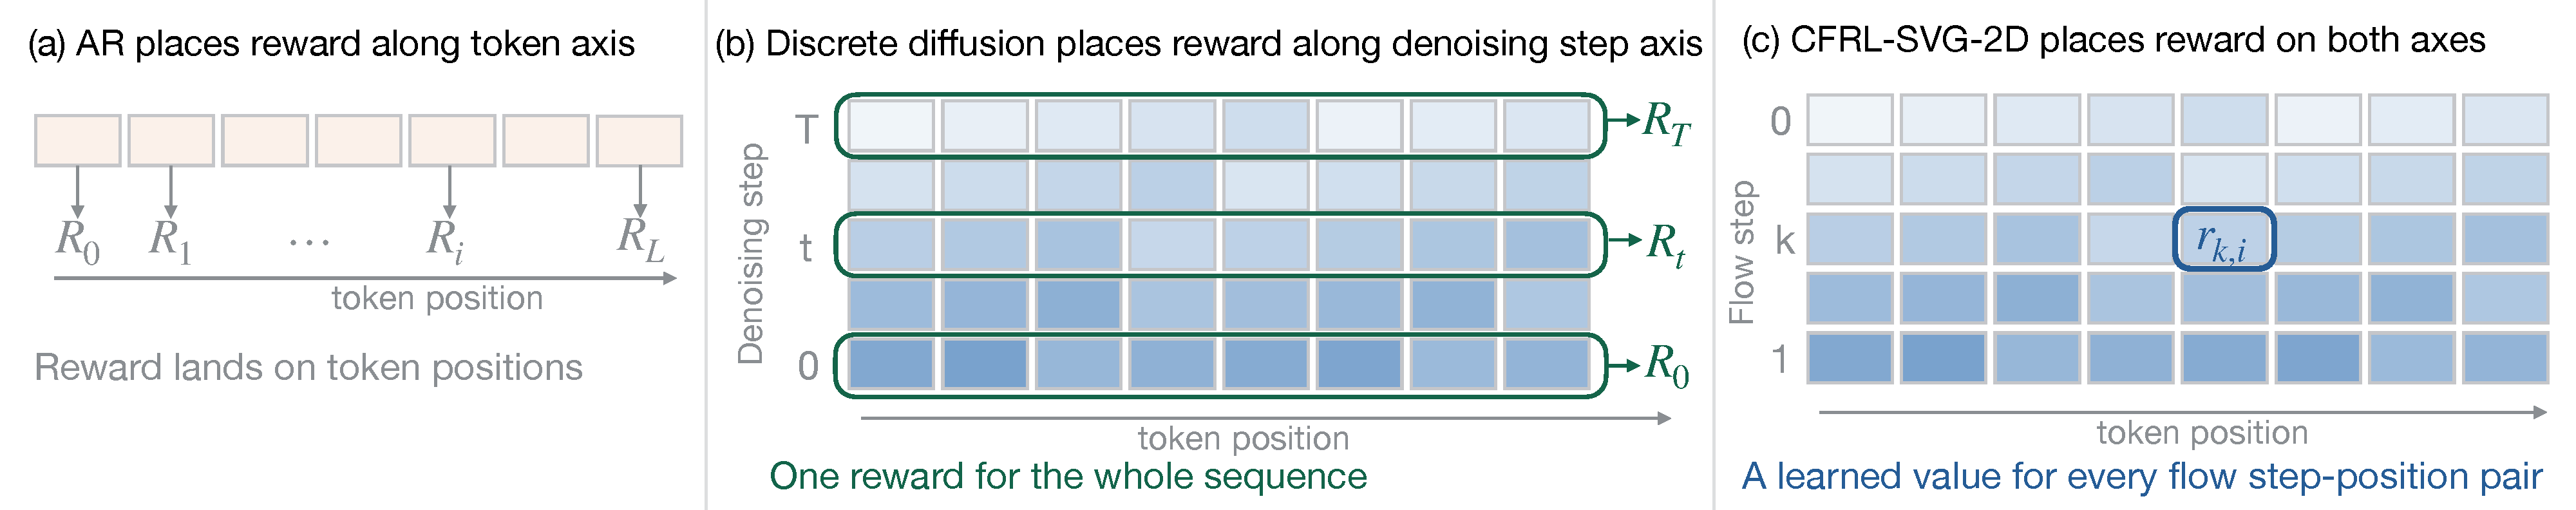
\includegraphics[width=0.78\linewidth]{figures/flow-rl-figure1.pdf}
\caption{(a) RL on AR models assigns reward over token positions (b) RL on discrete diffusions assigns reward over flow steps (c) \jpc{}-2D critic places reward on both flow steps and token positions.}
\label{fig:mechanism}
\end{figure}



\section{Amortising RL Gains Across Samplers}
\label{sec:loop}
A pathwise-trained policy realizes its largest gains under the sampler used during RL, and these gains may not transfer fully to cheaper samplers. We amortise them into the model through iterative verified self-training with Algorithm~\ref{alg:amortisation}. In each round, the current policy generates multiple candidates for a pool of training problems under the RL sampler. The verifier filters these candidates, and the policy is fine-tuned on the accepted samples using the original supervised objective. Successive rounds begin from the preceding round's checkpoint, allowing verified improvements to accumulate in the model parameters. The 2D critic can also guide candidate generation. At an intermediate flow step, its value field ranks partial states for pruning and supplies a gradient for improving the retained states before generation continues. This guidance helps maintain the coverage of verified samples when unguided sampling saturates. The resulting procedure is a form of rejection-sampling fine-tuning \citep{yuan2023rft,singh2023restem,zelikman2022star} adapted to continuous-state language models, transferring gains obtained with the RL sampler to less expensive deployment samplers.

\begin{algorithm}[t]
\caption{Amortising an RL policy by verified self-training}
\label{alg:amortisation}
\small
\begin{algorithmic}[1]
\REQUIRE initial RL policy $p_\theta^{(0)}$; verifier $r$; training prompt pools $\{\mathcal C_h\}_{h=1}^H$; RL sampler $\mathcal S$; cheaper sampler $\mathcal S'$; number of rounds $H$; candidates per prompt $N$; prune step $k_p$; pruning width $P$; optional critic $V_\phi$
\FOR{round $h=1,\dots,H$}
  \STATE Initialize the accepted set $\mathcal A_h\leftarrow\varnothing$
  \FOR{each prompt $c\in\mathcal C_h$}
    \FOR{candidate $n=1,\dots,N$}
      \IF{critic-guided sampling}
        \STATE Rollout trajectories up to step $k_p$: $\{\tau^j\}=\{(y_0, \dots, y_{k_p})^j\}_{j=1}^P \sim \mathcal S'(p_{\theta}^{(h-1)}(y\mid c))$ with normalized guidance during refinement: $y_{k} \leftarrow y_{k} \;+\; \lambda\,\sigma_{k}\,\sqrt{L}\,\frac{\nabla_{y}V_\phi(y_{k})}{\bigl\lVert\nabla_{y}V_\phi(y_{k})\bigr\rVert}$
        \STATE Prune at $k_p$: $\tau^*=\arg\max_j V_\phi(y^j_{k_p})$,  continue guided rollout to $K$, and decode to $w$
      \ELSE
        \STATE Draw a trajectory $\tau\sim \mathcal S(p_{\theta}^{(h-1)}(y\mid c))$ and decode to $w$
      \ENDIF
      \STATE Add accepted $w$ to $\mathcal A_h$: $\mathcal A_h \leftarrow \mathcal A_h \cup \{(c, w) \mid r(w,c)=1\}$
    \ENDFOR
  \ENDFOR
  \STATE Fine-tune from the current policy: $
    p_{\theta}^{(h)}
    \leftarrow
    \operatorname{SFT}
    \bigl(p_{\theta}^{(h-1)},\mathcal A_h; \mathcal L_{\mathrm{ELF}} \bigr)$
\ENDFOR
\RETURN amortised policy $p_\theta^{(H)}$
\end{algorithmic}
\end{algorithm}
\section{Experiments}
\label{sec:experiments}
\paragraph{Tasks.}
All four tasks have a program verifier, so rewards are exact and no reward model is involved (details in Appendix~\ref{app:datasets}). \textbf{Countdown} \citep{gandhi2024sos}: reach a target from four to five numbers with $+,-,\times,\div$; the answer is a derivation. \textbf{Sudoku} \citep{shah2024sudoku}: fill a $9\times9$ grid; solutions are unique; the model emits all 81 cells. \textbf{Knights-and-Knaves} (K\&K) \citep{xie2024kk}: assign knight/knave to $n\in\{4,5,6\}$ characters from their statements; solutions are unique. \textbf{Game24} \citep{yao2023tot}: reach 24 from four numbers. Game24 has only 1{,}345 solvable number sets, so we split by \emph{set}: the 1{,}601 evaluation prompts are orderings of 269 sets the model has never seen, and more supervised fine-tuning \emph{hurts} on this split (Appendix~\ref{app:g24_sft}).

\paragraph{Models and protocol.}
Every run starts from ELF-B (105M) fine-tuned on the task with the ELF recipe, at a checkpoint with headroom (Appendix~\ref{app:details}); accuracy is measured on 2{,}000 held-out prompts (1{,}601 for Game24) under four samplers (Appendix~\ref{app:results}), of which Table~\ref{tab:main} shows the deployment sampler ($\gamma56$@64; $\gamma28$@32 on Sudoku) and Table~\ref{tab:ode} the cheap 64-step ODE sampler. GRPO is the score-function baseline in its standard form (group size 8, uniform credit over steps and positions, no KL, 600 iterations, $\gamma4$@16 rollouts, checkpoints every 100). The two \jpc{} rows follow Algorithm~\ref{alg:jpc} exactly and differ only in the critic head: the scalar critic pools the features and then applies the head, the 2D critic applies the head at every position and pools the values; pre-training rollouts, stored steps, joint training, learning-rate schedule and evaluation are identical (1000--1500 iterations, a checkpoint every 250). Every ELF-B RL row is the mean over three seeds of the per-seed peak over all saved checkpoints, every seed counted (evaluation jitter $\approx\pm0.3$); the budgets differ by estimator (GRPO $\approx$77k rollouts of 16 steps per run, \jpc{} 32--48k rollouts of 64 steps plus the critic; comparable GPU-hours, Appendix~\ref{app:details}). GPT-2 (124M) and LLaDA-8B-Instruct are trained on the same data, with token-level GRPO/PPO and with d1's diffu-GRPO (Appendices~\ref{app:ar_curves} and~\ref{app:d1}). Every loop row starts from one policy and runs the same number of rounds per task (Countdown 4, Sudoku 1, K\&K 5, Game24 4); each round fine-tunes the previous round's final checkpoint on verifier-accepted samples of a fixed problem pool, and the tables report the last round (Appendix~\ref{app:details}).

\begin{table}[t]
\centering\small
\begin{minipage}[t]{0.585\linewidth}
\centering
\caption{Held-out accuracy (\%) at the deployment sampler.}
\label{tab:main}
\resizebox{\linewidth}{!}{%
\begin{tabular}{@{}lcccc@{}}
\toprule
 & Countdown & Sudoku & K\&K & Game24 \\
\midrule
\multicolumn{5}{@{}l}{\emph{GPT-2 (124M, autoregressive)}}\\
task SFT & 44.2 & \phantom{0}1.2 & 92.9 & 26.9 \\
+ token-level GRPO/PPO & 53.9 & \phantom{0}1.4 & 93.2 & 32.2 \\
\midrule
\multicolumn{5}{@{}l}{\emph{LLaDA-8B-Instruct (masked diffusion)}}\\
task SFT & 13.1 & \phantom{0}0.7 & 61.0 & 16.1 \\
+ diffu-GRPO & \PENDcd & \phantom{0}0.7 & 62.5 & 19.5 \\
\midrule
\multicolumn{5}{@{}l}{\emph{ELF-B (105M, continuous flow)}}\\
task SFT (base) & 42.2 & 66.2 & 67.5 & 45.0 \\
+ GRPO & 43.1 & 69.7 & 71.6 & 47.5 \\
+ \jpc{}, scalar critic & \textbf{48.5} & 67.4 & 78.2 & 51.9 \\
+ \hl{\jpc{}, 2D critic} & 46.9 & \textbf{70.0} & \textbf{79.2} & \textbf{58.9} \\
\midrule
\multicolumn{5}{@{}l}{\emph{ELF-B, amortisation loop (4 / 1 / 5 / 4 rounds)}}\\
loop from the SFT base (no RL) & \LOOPcdB & 65.5 & \LOOPkkB & 46.1 \\
loop from the GRPO policy & 45.1 & \textbf{71.9} & \LOOPkkG & 50.5 \\
gold labels of the loop's problems (oracle) & 43.1 & 70.5 & \textbf{99.8} & 49.5 \\
\hl{2D-critic policy + loop} & \textbf{52.3} & 70.8 & 98.8 & \textbf{58.1} \\
\bottomrule
\end{tabular}}
\end{minipage}\hfill
\begin{minipage}[t]{0.40\linewidth}
\centering
\caption{ELF-B at the cheap 64-step ODE sampler (\%).}
\label{tab:ode}
\resizebox{\linewidth}{!}{%
\begin{tabular}{@{}lcccc@{}}
\toprule
 & Countdown & Sudoku & K\&K & Game24 \\
\midrule
task SFT (base) & 28.1 & 62.3 & 57.8 & 35.2 \\
+ GRPO & 28.9 & \textbf{66.0} & 63.7 & 36.5 \\
+ \jpc{}, scalar critic & \textbf{33.5} & 64.3 & \textbf{69.1} & 38.6 \\
+ \hl{\jpc{}, 2D critic} & 33.3 & 65.2 & \textbf{69.1} & \textbf{41.2} \\
\midrule
loop from the SFT base & \LOOPcdBo & 62.0 & \LOOPkkBo & 40.2 \\
loop from the GRPO policy & 42.1 & \textbf{68.5} & \LOOPkkGo & 43.5 \\
gold labels (oracle) & 27.5 & 66.5 & \textbf{97.7} & 39.4 \\
\hl{2D-critic policy + loop} & \textbf{49.5} & 66.1 & 95.2 & \textbf{50.9} \\
\bottomrule
\end{tabular}}
\end{minipage}
\end{table}

\paragraph{Three levels of RL on the flow model.}
Table~\ref{tab:main} reads as three levels. \emph{Score-function (GRPO).} It works: every task improves at the deployment sampler, by $+3.5$ and $+4.1$ on Sudoku and K\&K, where the base already solves two thirds of the problems, but by only $+0.9$ on Countdown and $+2.5$ on Game24, the tasks with the most headroom. Its weaknesses are the ones \S\ref{sec:grpo} predicts for a noisy estimator: the gains are smallest where the headroom is largest, and where it does move the policy it is seed-sensitive (per-seed peaks spread over $6.6$ points on Sudoku, one seed never rising above the base). \emph{Pathwise with a scalar critic.} Under the same algorithm the pooled critic is already the stronger estimator where the headroom is large, $+6.3$ on Countdown, $+10.7$ on K\&K and $+6.9$ on Game24 over the base, but it is the less reliable one: on Sudoku every seed peaks by 500 iterations and then collapses to $51$--$54$, and it ends below GRPO there. \emph{Pathwise with the 2D critic.} Replacing the pooled value by the per-position field changes nothing else in the algorithm and adds $+2.6$ on Sudoku, $+1.0$ on K\&K and $+7.0$ on Game24; per-seed peaks agree within $0.5$--$1.5$ points on every task, every seed improves on the base and no run collapses within its schedule; it leads GRPO by $+7.6$ on K\&K and $+11.4$ on Game24, on every seed. Countdown is the exception: its field carries no information at the early and middle steps (Appendix~\ref{app:details}), the scalar head is $1.6$ ahead, and all three levels sit within $43$--$49$. The ODE sampler (Table~\ref{tab:ode}) orders the levels the same way: both critics lead GRPO on Countdown, K\&K and Game24, and Sudoku is the one column where GRPO's cheap-sampler accuracy is higher. The estimator matters where there is headroom, and the field is what makes it reliable.

\paragraph{The AR control.}
The score-function estimator is not weak in itself. A GPT-2 fine-tuned on the same data climbs from 44.2 to 53.9 on Countdown and from 26.9 to 32.2 on Game24 under token-level GRPO/PPO with textbook clip statistics, larger gains than any score-function variant achieves on the flow model (Table~\ref{tab:sf_variants}); on K\&K, where its supervised model already solves 92.9\%, and on Sudoku, where it solves 1\%, the same recipe leaves it where it started. Each architecture improves through the gradient channel its action space admits: the flow model gains $+13.9$ on Game24 through its native estimator. d1 \citep{zhao2025d1}, the standard recipe for masked diffusion models, run unchanged on our tasks and data, adds $1.5$--$3.4$ points to its supervised model on Countdown, K\&K and Game24 and never produces a solved Sudoku grid (Appendix~\ref{app:d1}).

\paragraph{The loop and its controls.}
The loop starts from the best 2D-critic seed of each task; the controls run the identical rounds from the SFT base, from the best GRPO seed, and from the 2D policy with the gold labels of the same pool problems in place of its own samples. On Countdown the loop is where the 2D policy pays off. Two plain rounds move the deployment sampler little ($47.5\!\to\!48.1$) while the ODE sampler gains ten points and the pool's coverage shrinks; rounds 3--4, whose pool is sampled with best-of-4 pruning and guidance by the jointly trained 2D critic, restore coverage (31k$\to$38k problems) and lift the deployment sampler to $52.3$ (Appendix~\ref{app:cd_loop}), against $\LOOPcdB$ from the base, $45.1$ from the GRPO policy and $43.1$ with gold labels. On Game24 four rounds take the ODE-64 sampler from $41.1$ to $50.9$ while the deployment sampler ends where it started ($59.3\!\to\!58.1$; Figure~\ref{fig:curves}, right): the loop transfers what the policy can do to the cheap sampler but does not raise a policy already at the ceiling of the split; the same rounds from the base, from the GRPO policy and on gold labels end at $46.1$, $50.5$ and $49.5$. On K\&K five rounds on fresh problems compound from $79.5$ to $98.8$ ($83.9$, $89.6$, $94.0$, $97.2$, $98.8$; ODE-64 from $69.5$ to $95.2$), one point below the gold-label chain ($99.8$); the loop compounds from the SFT base and from the GRPO policy as well ($\LOOPkkB$ and $\LOOPkkG$ after five rounds), so on K\&K the rounds, not the RL level, close the task: the loop is bounded by coverage, and any policy that solves a third of the pool climbs the same ladder (Appendix~\ref{app:kk_by_n}).

\paragraph{Where it does not help.}
Sudoku's loop is null from every start ($70.7\!\to\!70.8$ on 50k fresh puzzles from the 2D policy; $65.5$ from the base, $71.9$ from the GRPO policy's $72.8$, $70.5$ with gold labels): solutions are unique, so a policy only re-solves what it already solves, and the cheap samplers already sit within five points of the deployment one.

\begin{figure}[t]
\centering
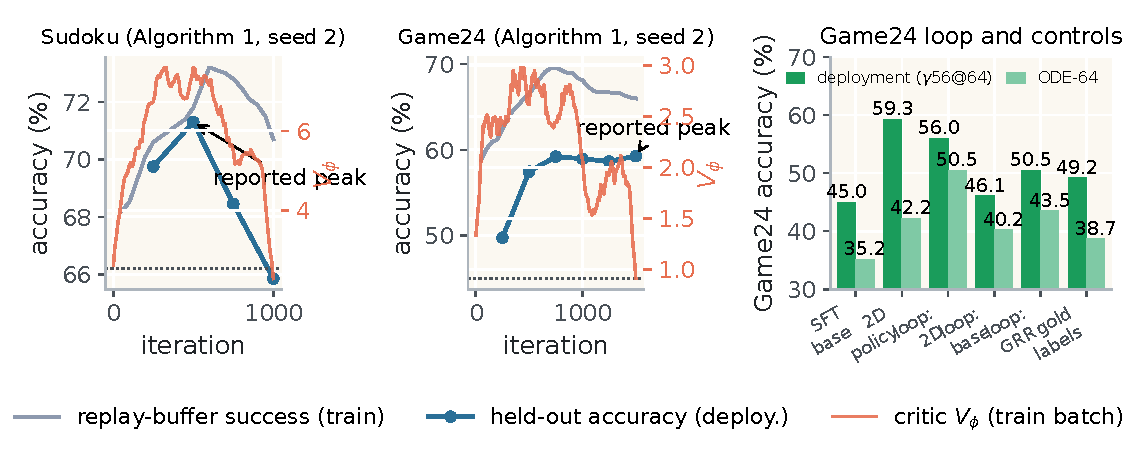
\includegraphics[width=0.66\linewidth]{figures/fig_dynamics_loop.pdf}
\caption{Left, middle: replay-buffer success (grey), critic value (red) and held-out accuracy (blue) for two \jpc{} runs; every run eventually enters a regime where the critic's value drifts while held-out accuracy falls, and the recipe keeps the held-out peak. Right: the loop on Game24 at the deployment and ODE-64 samplers (base, 2D-critic policy, loop from that policy, loop from the base).}
\label{fig:curves}
\end{figure}

\section{Ablations: what the design needs}
\label{sec:ablations}
The ablations remove one element of Algorithm~\ref{alg:jpc} at a time and read the result against the reason \S\ref{sec:joint} gave for it.

\paragraph{The critic must move with the policy.}
Figure~\ref{fig:frozen} shows the failure that~(\ref{eq:biasm}) predicts for a critic that is not refitted. With the critic frozen at its pre-trained weights, the pathwise update helps for 500 iterations on Game24 ($+3.4$ at 250, $+3.1$ at 500) and then finds the critic's blind spots: between iterations 500 and 800 the critic's value on the training batch climbs from $\approx3$ to $\approx90$ while the true success rate of the same batch falls to zero, and held-out accuracy falls to $2.1$ at 750. The identical run with two head steps per actor step on the replay buffer keeps the value in the calibrated range and reaches $+15.7$ (Table~\ref{tab:g24_abl}). One head step per actor step lags from 750 iterations on; eight match two; a buffer of 4k states matches 16k.

\paragraph{One chain.}
A policy trained under the cheap $\gamma4$@16 chain improves that chain by $+7.1$ but ends nine points below the deployment-trained policies at the deployment sampler (Table~\ref{tab:g24_abl}, last rows): the value, and with it the improvement, belongs to the chain it was defined on, which is why Algorithm~\ref{alg:jpc} trains under the sampler that will be deployed and why \S\ref{sec:loop} is needed for the others.

\paragraph{Which states the critic learns from.}
The head is refitted on the state at the top of the window only. An earlier version of the recipe stored five evenly spaced steps of the window instead. On Countdown, where the pre-trained critic's held-out AUC is $0.64$ at steps $8$--$24$ of 64 and $0.90$ at step 40, fitting the early states cost the 2D critic three points ($46.9/46.0/47.5$ against $50.1/50.2/50.4$ over three seeds), while on Sudoku, K\&K and Game24 the two versions agree within a point ($70.0/79.2/58.9$ against $71.0/79.6/58.8$). The pre-training of the copy is the other lever. On K\&K, with Algorithm~\ref{alg:jpc} otherwise unchanged (five-step buffer), a critic pre-trained on 16k rollouts at five stored steps for six epochs gives $71.2/72.0/70.6$ and collapses by 500 iterations; the same critic pre-trained on 32k rollouts at seven steps for ten epochs gives $79.5/79.1/79.0$. The pooled value's correlation with the outcome barely changed between the two ($0.70$ against $0.71$ on held-out rollouts), but the correlation of the minimum per-position value rose from $0.38$ to $0.66$: the actor uses the field, not only its mean. The same budget did not change the other tasks, whose critics were already sharp (Appendix~\ref{app:details}).

\paragraph{Step size.}
At an actor learning rate of $3\times10^{-6}$ the 2D critic reaches the level of Table~\ref{tab:main} within 250 iterations and then collapses, on Countdown from $50.1$ to $28.5$ and on Game24 from $58.0$ to $30.3$ by iteration 1000; the scalar critic at the same rate is seed-fragile (Appendix~\ref{app:lr_regime}). At $10^{-6}$ every 2D run of Table~\ref{tab:main} holds, and with the cosine decay none declines before its last checkpoint. The bias~(\ref{eq:biasm}) is paid per step, and the step is the one setting that separates a run that holds from one that collapses.

\paragraph{The rest changes speed, not level.}
With the pooled loss term alone, or without the AUC safeguard, single Game24 runs reach $59.0$ and $58.7$ against $58.9$ for the full recipe but sit $2$--$4$ points lower at 500 iterations (Appendix~\ref{app:details}).

\begin{figure}[t]
\centering
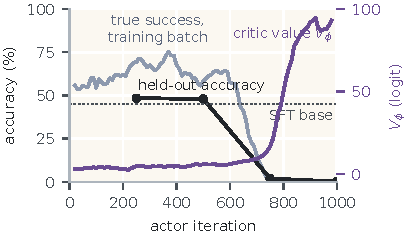
\includegraphics[width=0.9\linewidth]{figures/fig_frozen.pdf}
\caption{Frozen against jointly trained critic on Game24 (2D critic, $10^{-6}$). Red: the critic's value on the training batch; grey: the true success rate of that batch; blue: held-out accuracy at the deployment sampler. With a frozen critic the value is driven to $\approx90$ while success collapses to zero; with the head refitted after every actor step the value stays calibrated and the policy improves.}
\label{fig:frozen}
\end{figure}

\begin{table}[t]
\centering\small
\caption{Game24 ablations of joint training (2D critic, $10^{-6}$): held-out accuracy at $\gamma56$@64 by iteration (base $45.0$) and ODE-64 accuracy at the best checkpoint (base $35.2$). Reference row: mean of three seeds; other rows: single runs. The last two rows are one run trained under $\gamma4$@16, read at two samplers.}
\label{tab:g24_abl}
\resizebox{\linewidth}{!}{%
\begin{tabular}{@{}lccccc@{}}
\toprule
variant & @250 & @500 & @750 & @1000 & ODE-64 (best) \\
\midrule
frozen critic (no refit) & 48.4 & 48.0 & \phantom{0}2.1 & \phantom{0}0.3 & 38.0 \\
critic steps $m_{\rm c}{=}1$ & 48.0 & 51.7 & 48.6 & 51.1 & 40.3 \\
critic steps $m_{\rm c}{=}8$ & 47.0 & 52.3 & 54.7 & 55.2 & 40.5 \\
buffer $N_{\mathcal B}{=}4$k & 47.8 & 50.1 & 52.6 & 56.4 & 42.4 \\
trained under $\gamma4$@16, read at $\gamma56$@64 & 44.7 & 44.3 & 41.5 & 47.0 & 36.7 \\
trained under $\gamma4$@16, read at $\gamma4$@16 & 35.1 & 38.7 & 41.3 & 42.5 & --- \\
\midrule
\hl{Algorithm~\ref{alg:jpc} ($m_{\rm c}{=}2$, $N_{\mathcal B}{=}16$k, deployment chain)} & 48.7 & 50.9 & 53.0 & 56.4 & 42.0 \\
\bottomrule
\end{tabular}}
\end{table}

\section{Related work}
\label{sec:related}
Continuous-state language models go back to Diffusion-LM \citep{li2022diffusionlm}; ELF \citep{hu2026elf} removes intermediate discretisation with flow matching \citep{lipman2022flow,liu2022rectified,albergo2023stochastic} in a frozen embedding space. Masked diffusion language models \citep{lou2023sedd,sahoo2024mdlm,nie2025llada} have an RL literature built on likelihood surrogates \citep{zhao2025d1,zhu2025llada15}, none of which applies to a differentiable chain. RL for image diffusion and flows splits into score-function methods \citep{black2023ddpo,fan2023dpok,liu2025flowgrpo,xue2025dancegrpo,li2025mixgrpo}, likelihood-surrogate policy gradients \citep{mcallister2025fpo}, and reward back-propagation through a fixed differentiable reward \citep{prabhudesai2023alignprop,clark2023draft,domingoenrich2024adjoint}; our critic is learned from a non-differentiable verifier and trained jointly, as in actor-critic control \citep{lillicrap2015ddpg,haarnoja2018sac}. AR post-training with verifiable rewards \citep{ouyang2022instructgpt,shao2024deepseekmath,deepseek2025r1,yu2025dapo,zheng2025gspo} is the estimator we port; the amortisation loop is rejection-sampling fine-tuning \citep{yuan2023rft,singh2023restem,zelikman2022star,huang2022selfimprove,anthony2017exit} with an RL policy as sampler (Appendix~\ref{app:related}).

\section{Conclusion}
We propose \method{}, RL post-training for continuous flow language models in three variants and an amortisation loop. \methodGRPO{} is the score-function estimator on the chain's exact density; \methodSVGScalar{} and \methodSVGTwoD{} are stochastic value gradients with one value per state, or per state and token position. \methodGRPO{} gains little: one reward bit is spread over the chain's noise coordinates, and its gradient agrees with itself no better than a zero-mean control, whereas GPT-2's gradient, with one score term per token decision, does. Differentiating the chain through a critic removes the noise factor. The critic must read the denoiser's estimate through a copy of the pre-trained denoiser and be refit after every actor step, or it is exploited. With one value per position the policy rises faster and further than with a scalar value, and exchanging the critics mid-training shows that the critic in charge decides. The loop carries the gain into a cheap chain. \emph{Limitations:} one 105M architecture and four synthetic tasks with exact verifiers.


\subsubsection*{Reproducibility statement}
Code, configurations and job scripts for every run in this paper will be released; all datasets are generated programmatically or drawn from public collections (Appendix~\ref{app:datasets}) and the exact splits, seeds and verifier implementations are included. Appendix~\ref{app:datasets} defines the samplers, Appendix~\ref{app:details} lists every hyperparameter, the evaluation protocol and the compute used; Appendix~\ref{app:results} reports the full trajectories and the supporting results behind the numbers in the main text.

\subsubsection*{AI use statement}
In this work, we used generative AI tools for writing assistance (editing prose), for writing and debugging experiment code. We have not used generative AI tools for generating research ideas that are presented as contributions, nor for producing any experimental result, number or figure that was not computed by the released code. We have reviewed all AI-assisted work: all code was tested against the reported runs, all citations were verified against the cited sources, and all claims were checked against the experiment logs. The authors take full responsibility for all content of this paper.


\bibliography{refs}
\bibliographystyle{iclr2027_conference}

\appendix
\section{Datasets and verifiers}
\label{app:datasets}
All tasks are generated programmatically; every prompt has a program verifier that decides correctness of a model output without reference to the gold answer, so rewards are exact and label-free.

\paragraph{Countdown.}
Following the Countdown formulation of \citet{gandhi2024sos}, a prompt is four or five integers and a target; the model emits a derivation as a sequence of binary operations (\texttt{12-5=7 , 4*7=28 , 28-3=25} for the numbers 12, 5, 4, 3 and the target 25). The verifier parses the derivation, checks that every operation is arithmetically correct, that each input number is used at most once, and that the last result equals the target. The supervised set is 500k examples, one gold derivation each; the loop's pool is a disjoint set of 50k unlabelled problems; evaluation uses 2{,}000 held-out problems. Sequence length is 72 embedding positions (16 for the condition).

\paragraph{Sudoku.}
Puzzles are drawn from a public collection of rated Sudoku puzzles (with solutions); the model reads the 81-cell puzzle (blanks as \texttt{*}) and emits all 81 cells. The verifier checks that the output is a valid grid consistent with the givens; since solutions are unique this equals exact match. The supervised set is 400k puzzles, evaluation 2{,}000 held-out puzzles; the ``fresh puzzle'' pool for the loop is 50k further puzzles with no overlap with training, validation or test. Sequence length is 164 (82 condition, 82 target).

\paragraph{Knights-and-Knaves.}
Following \citet{xie2024kk}, each puzzle has $n\in\{4,5,6\}$ characters who each make one statement (``A: C knave'', ``B: A same C'', ``C: D diff B''); the model outputs an assignment (``A knight B knave \dots''). Our generator enumerates assignments and keeps only puzzles with a unique solution; the verifier re-parses the statements and checks that the assignment satisfies every one. Training uses 300k puzzles; evaluation 2{,}000; the loop's first round samples the 50k training puzzles without their labels, and every later round a fresh 50k pool disjoint from training, validation and each other. The supervised model reaches 96.8/93.8/99.4/99.7 (ODE-64/$\gamma4$@16/$\gamma28$@32/$\gamma56$@64) at epoch 8, so the RL base is the epoch-4 checkpoint (57.8/58.1/65.8/67.5) and the epoch-8 model is the supervised oracle. Sequence length is 96 (56 condition).

\paragraph{Game24.}
Following the Game of 24 of \citet{yao2023tot}, reach 24 from four numbers in $\{1,\dots,13\}$ with each number used once. Only 1{,}345 unordered number sets are solvable, so we split by set: the training set contains 13{,}150 orderings of 1{,}076 sets with one gold derivation each, the loop pool a further 4{,}693 orderings of the training sets, and the evaluation set 1{,}601 orderings of the 269 remaining sets, which the model never sees in any order. The verifier is the Countdown verifier with target 24. Sequence length is 72 (16 condition). The supervised model is initialised from the Countdown model and trained for 40 epochs; held-out accuracy peaks at epoch 20 (35.2/35.4/42.6/45.0 at ODE-64/$\gamma4$@16/$\gamma28$@32/$\gamma56$@64) and falls to 30.5/29.8/32.1/34.7 by epoch 40, so the epoch-20 checkpoint is the RL base and there is no supervised oracle above it.

\paragraph{Samplers.}
ODE-64 is the 64-step deterministic sampler of \citet{hu2026elf}. $\gamma56$@64 denotes the SDE sampler of~\eqref{eq:chain} with $K{=}64$ uniform steps and churn $\gamma{=}56$, and likewise for the other values; $\gamma56$@64, $\gamma28$@32 and $\gamma14$@16 all have per-step retention $\alpha\approx0.125$, which we found to be the best sampling configuration independently of $K$ (more steps still help at fixed $\alpha$); $\gamma4$@16 is a cheap low-churn configuration. All evaluations use classifier-free guidance 2 and self-conditioning guidance 1 as in the ELF release. Throughout, the \emph{deployment chain} is $\gamma56$@64 ($\gamma28$@32 on Sudoku) and the \emph{cheap chain} is $\gamma4$@16 ($\gamma14$@16 on Sudoku).

\section{Derivations}
\label{app:derivations}
\subsection{Exact transition kernels of the SDE sampler}
ELF's stochastic sampler at step $k$ with step size $h_k$ and churn $\gamma$ predicts $\hat x_k=D_\theta(y_{k-1},t_{k-1},c)$, moves towards it, and re-noises: $y_k=(1-\gamma h_k)\,\hat x_k+\gamma h_k c_\sigma\,\varepsilon_k$ with $\varepsilon_k\sim\mathcal N(0,I)$ and $c_\sigma$ the noise scale of the interpolant at the target time (we absorb the deterministic drift terms into $D_\theta$; the released code is the reference). Indexing the chain by the post-noising iterates $y_k$ gives $p_\theta(y_k\mid y_{k-1})=\mathcal N(y_k;\alpha_kD_\theta(y_{k-1}),\sigma_k^2I)$ with $\alpha_k=1-\gamma h_k$ and $\sigma_k=\gamma h_kc_\sigma$, and the final decode $p(w\mid y_K)=\prod_i\mathrm{Cat}(w_i;\mathrm{softmax}(E\,D_\theta(y_K)_i))$ with $E$ the embedding matrix. The trajectory log-likelihood is the sum of these terms and requires no bound. We verified the implementation on CPU: recomputing the log-probability of a stored trajectory under the same parameters agrees with the value recorded at rollout to relative error $7\times10^{-5}$ (flow steps) and $10^{-3}$ (decode). Two caveats that matter in practice: $\gamma h_k\ge1$ makes $\alpha_k=0$ and every parameter gradient exactly zero (we assert $\alpha_k>0$), and storing states in bfloat16 perturbs summed log-ratios by $O(1)$ over $L\times d$ dimensions, so ratio-based estimators need per-dimension normalisation or fp32 storage.

\subsection{Score-function and pathwise gradients}
\label{app:variance}
For~(\ref{eq:chain}), $\nabla_\theta\log\mathcal N(y_k;\alpha_kD_\theta,\sigma_k^2I)=\sigma_k^{-2}(y_k-\alpha_kD_\theta)^{\top}\alpha_k\partial D_\theta/\partial\theta=\sigma_k^{-1}\varepsilon_k^{\top}\alpha_k\,\partial D_\theta/\partial\theta$, which is~(\ref{eq:sf}). The estimator's variance is that of a sum of $K\cdot L\cdot d$ terms each proportional to an independent standard normal, weighted by an advantage that depends on the trajectory only through the final reward. Write the reward as a function of the noise path, $r=r(\varepsilon_{1:K})$; the score-function estimate of $\partial_\theta\mathbb E[r]$ is $\mathbb E[r\sum_k\sigma_k^{-1}\varepsilon_k^{\top}\alpha_kJ_k]$ with $J_k=\partial D_\theta/\partial\theta$, so a coordinate contributes signal only through the covariance of $r$ with that coordinate's noise. In an AR model the analogous decomposition has one term per token and every term is a categorical decision the reward depends on; in the flow model, 86\% of positions are decided at the first step and never change (\S\ref{app:commit}), so almost every coordinate at almost every step has vanishing covariance with $r$ while contributing its full variance. With $N$ trajectories the signal scales as $N$ times the few informative covariances and the noise as $\sqrt{N\cdot K L d}$; the ratio of informative to total coordinates ($\sim$30 semantic decisions against $5\times10^{5}$--$2\times10^{6}$ coordinates) is the $10^{4}$--$10^{5}$ gap quoted in \S\ref{sec:estimators}. Refining the advantage (per-step, per-position, oracle) changes which coordinates receive weight but not this ratio, which is why Table~\ref{tab:sf_variants} is flat.

The pathwise estimator uses the same reparameterisation: $y_k$ is a deterministic function of $(\theta,\varepsilon_{1:k})$, so for a differentiable surrogate $V_\phi$ of $\mathbb E[r\mid y_k]$, $\partial_\theta V_\phi(y_k)=\partial_{y}V_\phi\cdot\alpha_k\,\partial_\theta D_\theta(y_{k-1})$ holds coordinate-wise with no noise factor. Its bias is that of the critic, which is why the critic must track the policy. We use one random $k$ per trajectory (the ``one-step'' variant) rather than back-propagating through the whole chain as in \citet{prabhudesai2023alignprop,clark2023draft}; with a critic on intermediate states the chain need not be differentiated, and memory is constant in $K$.

\subsection{Why the pathwise update ascends the reward: derivation of~(\ref{eq:pw})}
\label{app:pw_derivation}
This section derives the pathwise update of \S\ref{sec:estimators} from the objective~(\ref{eq:objective}) and makes precise in what sense the one-step \jpc{} update of \S\ref{sec:method} is a policy-gradient step on the expected reward. Fix a prompt $c$ and drop it from the notation. The chain~(\ref{eq:chain}) is $y_0=c_\sigma\varepsilon_0$ and $y_k=\alpha_kD_\theta(y_{k-1})+\sigma_k\varepsilon_k$ for $k=1,\dots,K$ with $\varepsilon_0,\dots,\varepsilon_K$ independent standard Gaussians, and the reward is a function of the last state, $r(y_K):= r(w(y_K),c)$, where $w(y_K)$ is the decoded text (the final ODE step and the decoder head are absorbed into this map).

\paragraph{Value functions.}
For $k=0,\dots,K$ define the value of a state at flow step $k$ under the current policy,
\begin{equation}
V_k(y):=\mathbb E\big[r(y_K)\,\big|\,y_k=y\big],
\label{eq:valuedef}
\end{equation}
where the expectation is over the remaining noise $\varepsilon_{k+1},\dots,\varepsilon_K$. Then $V_K=r$, the objective is $J(\theta)=\mathbb E[V_0(y_0)]$, and the tower property gives the one-step recursion
\begin{equation}
V_{k-1}(y)=\mathbb E_{\varepsilon_k}\big[V_k\big(\alpha_kD_\theta(y)+\sigma_k\varepsilon_k\big)\big].
\label{eq:bellman}
\end{equation}
Every $V_k$ with $k<K$ depends on $\theta$ through the downstream transitions; $V_K=r$ does not. The 1D critic of \S\ref{sec:method} is a learned approximation of $V_k$, and the 2D critic is a learned approximation of $V_k$ that is additive over the positions of $y$.

\paragraph{Step 1: the policy gradient is a sum over transitions.}
$J$ depends on $\theta$ through each of the $K$ transitions. Give the $k$-th transition its own copy $\theta_k$ of the parameters, so that $J=J(\theta_1,\dots,\theta_K)$ with all copies tied to $\theta$; by the chain rule,
\begin{equation}
\nabla_\theta J=\sum_{k=1}^{K}\frac{\partial J}{\partial\theta_k}\Big|_{\theta_1=\dots=\theta_K=\theta}.
\label{eq:sumover}
\end{equation}
This is the decomposition behind every per-step estimator, including the score-function form~(\ref{eq:sf}): writing the $k$-th transition density as $\mathcal N(y_k;\alpha_kD_{\theta_k}(y_{k-1}),\sigma_k^2I)$ and applying the likelihood-ratio identity to the expectation of the downstream value gives
\begin{equation}
\frac{\partial J}{\partial\theta_k}=\mathbb E\Big[V_k(y_k)\,\nabla_{\theta_k}\log\mathcal N\big(y_k;\alpha_kD_{\theta_k}(y_{k-1}),\sigma_k^2I\big)\Big]=\mathbb E\Big[V_k(y_k)\,\frac{\varepsilon_k^{\top}}{\sigma_k}\,\alpha_k\frac{\partial D_\theta(y_{k-1})}{\partial\theta}\Big],
\label{eq:sfterm}
\end{equation}
and replacing $V_k(y_k)$ by the Monte-Carlo return $r(y_K)$, or by an advantage $V_k(y_k)-b(y_{k-1})$ with any baseline $b$, leaves the expectation unchanged because $\mathbb E[\varepsilon_k\mid y_{k-1}]=0$. Summing~(\ref{eq:sfterm}) over $k$ and over the positions of $y_k$ is~(\ref{eq:sf}).

\paragraph{Step 2: the pathwise form of the same term.}
Condition on $y_{k-1}$ and use the reparameterisation $y_k=\alpha_kD_{\theta_k}(y_{k-1})+\sigma_k\varepsilon_k$. The objective depends on $\theta_k$ only through $y_k$, and the downstream value $V_k$ does not depend on $\theta_k$, so
\begin{equation}
\frac{\partial J}{\partial\theta_k}=\mathbb E\Big[\frac{\partial}{\partial\theta_k}V_k\big(\alpha_kD_{\theta_k}(y_{k-1})+\sigma_k\varepsilon_k\big)\Big]=\mathbb E\Big[\sum_{i=1}^{L}\frac{\partial V_k(y_k)}{\partial y_{k,i}}\,\alpha_k\,\frac{\partial D_\theta(y_{k-1})_i}{\partial\theta}\Big],
\label{eq:pwterm}
\end{equation}
which is exactly~(\ref{eq:pw}) with the critic $V_\phi$ replaced by the true value $V_k$. Exchanging derivative and expectation is legitimate for $k<K$ because, by~(\ref{eq:bellman}), $V_k$ is a Gaussian smoothing of a bounded function composed with $D_\theta$, hence as smooth as $D_\theta$ and with bounded gradient. For $k=K$ it is not: $V_K=r$ is piecewise constant in $y_K$ (the decode is an $\arg\max$ and the verifier a program), so its almost-everywhere gradient is zero and the pathwise identity carries no signal through the final transition. This is the precise sense in which ``the reward itself is not differentiable'' in \S\ref{sec:estimators}, and why the pathwise route needs a value estimate on \emph{intermediate} states rather than the reward on the final one. \emph{Conclusion of Steps 1--2:} with an exact critic, (\ref{eq:pw}) evaluated at step $k$ is an unbiased estimate of $\partial J/\partial\theta_k$, the $k$-th transition's contribution to the gradient of the expected reward.

\paragraph{Step 3: (\ref{eq:pw}) is~(\ref{eq:sf}) with the noise integrated out.}
The two forms of $\partial J/\partial\theta_k$ are related by Gaussian integration by parts (Stein's identity): for $\varepsilon\sim\mathcal N(0,I_n)$ and any $f$ that is almost-everywhere differentiable with $\mathbb E|f|,\mathbb E\|\nabla f\|<\infty$,
\begin{equation}
\mathbb E\big[f(\mu+\sigma\varepsilon)\,\varepsilon\big]=\sigma\,\mathbb E\big[\nabla f(\mu+\sigma\varepsilon)\big].
\label{eq:stein}
\end{equation}
With $f=V_k$, $\mu=\alpha_kD_\theta(y_{k-1})$ and $\sigma=\sigma_k$, (\ref{eq:stein}) turns the score-function factor $V_k(y_k)\,\varepsilon_k/\sigma_k$ of~(\ref{eq:sfterm}) into the pathwise factor $\nabla_yV_k(y_k)$ of~(\ref{eq:pwterm}), conditionally on $y_{k-1}$. The two estimators therefore have the same expectation and differ only in variance, and the difference is visible coordinate by coordinate: the score-function factor at coordinate $(k,i)$ is $V_k(y_k)\,\varepsilon_{k,i}/\sigma_k$, a random variable of variance $\approx\mathbb E[V_k^2]/\sigma_k^2$ whether or not the coordinate affects the reward, whereas the pathwise factor is $\partial V_k/\partial y_{k,i}$, which is identically zero on every coordinate the value does not depend on. This is the variance argument of Appendix~\ref{app:variance} in one identity: the noise factor that integration by parts removes is the same factor that makes~(\ref{eq:sf}) average each reward bit over the $K\cdot L\cdot d$ coordinates of the trajectory.

\paragraph{Step 4: one random flow step.}
\jpc{} draws one $k$ uniformly from a window $\mathcal W=\{k_0,\dots,k_1\}$ and applies~(\ref{eq:pw}) at that step. Taking the expectation over $k$,
\begin{equation}
\mathbb E_{k\sim\mathcal U(\mathcal W)}\big[\hat g_{\mathrm{PW},k}\big]=\frac1{|\mathcal W|}\sum_{k\in\mathcal W}\frac{\partial J}{\partial\theta_k},
\label{eq:window}
\end{equation}
so the one-step update is, up to the constant $|\mathcal W|$, an unbiased Monte-Carlo estimate of the window's share of~(\ref{eq:sumover}). The transitions outside the window contribute little to~(\ref{eq:sumover}): at the earliest steps the state is dominated by noise and $V_k$ is nearly flat (the pooled critic value is at chance for $k\lesssim K/8$, Table~\ref{tab:critic_quality}), and at the last steps the state is committed and $V_k\to r$ is piecewise constant, with zero gradient almost everywhere. Restricting to the window therefore drops terms that are small or exactly zero, and it is what makes the update's memory independent of $K$: the downstream dependence of the reward on $y_k$ is carried by $V_k$ in expectation, through~(\ref{eq:bellman}), not by back-propagating through the remaining $K-k$ network evaluations as in reward back-propagation for image diffusion. Differentiating through $m$ consecutive transitions instead would recover the sum of $m$ consecutive terms of~(\ref{eq:sumover}) by the chain rule through the intermediate $D_\theta$; we found no benefit from this (Appendix~\ref{app:results}), consistent with the terms being individually estimable.

\paragraph{Step 5: the learned critic, and why it must be trained jointly.}
Replacing $V_k$ by the critic $V_\phi$ in~(\ref{eq:pwterm}) adds the bias
\begin{equation}
\mathbb E\Big[\sum_i\frac{\partial\,(V_\phi-V_k)(y_k)}{\partial y_{k,i}}\,\alpha_k\frac{\partial D_\theta(y_{k-1})_i}{\partial\theta}\Big],
\label{eq:bias}
\end{equation}
so the update ascends $J$ to the extent that the critic's slope matches the true value's slope on the states the current policy visits. Two things move that target as $\theta$ changes: the distribution of $y_k$ under the policy, and $V_k$ itself, which by~(\ref{eq:bellman}) is a function of the downstream policy, so a critic fitted to an older policy is wrong even at the same state. Both are why the critic is refitted on the current policy's own rollouts after every actor step (\S\ref{sec:method}); training it by binary cross-entropy on the verifier outcome fits $\sigma(V_\phi)$ to $\mathbb E[r\mid y_k]$, i.e.\ to~(\ref{eq:valuedef}) up to the logistic link. Equation~(\ref{eq:bias}) also describes the failure mode: wherever $V_\phi-V_k$ has a positive slope the actor ascends $V_\phi$ while the true expected reward is flat or falls, which is the frozen-critic exploit of Appendix~\ref{app:frozen}, and the reason the recipe stops at the held-out peak.

\subsection{Token commitment along the trajectory}
\label{app:commit}
For each generated position we record the first step at which the denoiser's prediction $\hat x_k$ decodes to the final token and never changes afterwards. On Countdown, 86\% of positions commit at step 0 (median 0, 90th percentile 2), identically for $\gamma\in\{4,8,14\}$; the remaining contested positions commit uniformly along the trajectory. Word decisions therefore live in the first forward pass and in the self-conditioned prediction channel, not in the noise.

\section{Experimental details}
\label{app:details}

\paragraph{Base models.}
ELF-B \citep{hu2026elf}: 105M-parameter transformer denoiser, frozen T5-small \citep{raffel2020t5} encoder embeddings ($d{=}512$), x-prediction with self-conditioning and training-time classifier-free guidance, PyTorch port of the released code. Supervised fine-tuning uses the released recipe (AdamW, learning rate $2\times10^{-3}$ with warm-up, global batch 256--512, EMA of weights; EMA decay 0.99 for the short Game24 run and 0.999 otherwise). The Countdown base is epoch 60 of a 100-epoch run; Sudoku uses the converged model (76 epochs on 400k puzzles); K\&K the epoch-4 checkpoint of a 40-epoch schedule stopped at epoch 9; Game24 the epoch-20 checkpoint of a 40-epoch run initialised from the Countdown model.

\paragraph{Critic.}
The critic reuses the denoiser architecture as a feature extractor (a copy of the trunk, fine-tuned at $10^{-5}$), takes the noisy state $y$, the time $t$ and the self-conditioning prediction $\hat x$ as input, and applies a per-position MLP head ($d{+}1\to256\to64\to1$, GELU) to produce $R_i$; the value is the mean of $R_i$ over generated positions. Pre-training data: 16k--32k rollouts of the base policy under the deployment sampler with states stored at $k\in\{1,8,16,32,48\}$ of 64 (or $\{1,8,16,24\}$ of 32), 6 epochs, batch 64, BCE on the verifier outcome. Pre-trained critics reach a top-1 selection accuracy (pick@$V$) that rises from 0.57 at $k{=}1$ to 0.99 at $k{=}48$ against a random baseline of 0.53 on Game24, and similarly on the other tasks.

\paragraph{\jpc{}.}
32 prompts per iteration, deployment sampler rollouts without gradients, one random step $k\in[8,40]$ of 64 (or $[4,20]$ of 32) recomputed with gradients, loss $-V_\phi(y_k)$ averaged over prompts, AdamW on the actor with gradient clipping at 1.0, learning rate $10^{-6}$ (2D critic) or $3\times10^{-6}$ for 500 iterations followed by $10^{-6}$ for 250 with actor and critic resumed (scalar critic). Critic: replay buffer of 16{,}384 trajectories (4{,}096 for the scalar critic) with states at the stored $k$, 2 gradient steps per iteration, batch 64, learning rate $10^{-5}$, BCE on the outcome. Checkpoints every 250 iterations (125 for refinement phases) evaluated on the full held-out set; the reported checkpoint is the held-out peak. Runs take 45--90 minutes for 1000 iterations on one H200 (2--3 hours on an A100-40G).

\paragraph{GRPO.}
Group size 8, 16 prompts per iteration (128 rollouts), $\gamma4$@16 rollouts, uniform credit over steps and positions, group-normalised advantage, no KL, no clipping (on-policy REINFORCE form; the clipped per-position variant is in Table~\ref{tab:sf_variants}), learning rate $3\times10^{-6}$, 8 transitions per update, 600 iterations, checkpoints every 100 evaluated on the held-out set with the peak reported. Three seeds per task.

\paragraph{AR control.}
GPT-2 (124M) fine-tuned on the Countdown training set for 10 epochs (batch 128, learning rate $3\times10^{-4}$, warm-up 500) reaches 44.2\% on the 2{,}000 held-out problems with greedy decoding; token-level GRPO/PPO with 32 prompts $\times$ 8 samples, clip 0.2, no KL, 2 inner epochs and learning rate $10^{-5}$ reaches 53.9\% at iteration 550 (evaluated every 50 iterations). For Game24 the same GPT-2 (initialised from the Countdown-fine-tuned weights, as the flow model is) reaches 26.9\% on the set-split evaluation after SFT and 32.2\% after 600 RL iterations.

\paragraph{Amortisation loop.}
Pool sampling uses the deployment sampler on a pool of training-side problems (Countdown: a disjoint unlabelled pool; Game24: the 4{,}693 pool orderings, 8 seeds each; K\&K: 50k fresh problems, 2 seeds; Sudoku: 50k training or fresh puzzles, 2--4 seeds), keeps verifier-accepted samples with at most four (Countdown, Game24) or one (unique-solution tasks) per problem, and fine-tunes with the supervised recipe for 8 epochs from the current policy. The gold controls use the same schedule and initialisation with gold labels. On Countdown, rounds 3--4 sample the pool with critic-guided sampling (critic best-of-4 pruning at step 32 and critic gradient guidance) to restore pool coverage; every other pool is sampled with the plain deployment sampler (Appendix~\ref{app:cd_loop}).

\paragraph{Evaluation and seeds.}
Every number is one evaluation of 2{,}000 held-out prompts (1{,}601 for Game24) at classifier-free guidance 2 with a fixed sampler seed; cross-GPU jitter of the same checkpoint is $\approx\pm0.3$ points. Seeds change the rollout noise and prompt order; per-seed peaks are reported with their standard deviation. \emph{Number of runs behind Table~\ref{tab:main}.} GRPO: three seeds on Sudoku, K\&K and Game24, and three on Countdown (in progress at the time of writing; the Countdown entry of Table~\ref{tab:sf_variants} is a single run of a different variant). \jpc{} scalar critic: three seeds on Countdown ($51.2/49.2/42.8$), two on Sudoku ($53.1/58.1$, both collapsing by 500 iterations) and Game24 ($55.2/39.5$), one on K\&K ($70.5$), with the missing seeds in progress. \jpc{} 2D critic: three seeds on Sudoku ($69.9/70.1/69.2$), K\&K ($70.3/70.3/70.8$) and Game24 ($56.8/60.6/58.8$), two on Countdown ($48.4/47.3$, third in progress). Every loop row, the AR control and the LLaDA rows are single runs. Per-seed values at all four samplers are in Appendix~\ref{app:results}.

\paragraph{Compute.}
The campaign used about 300 GPU-hours on A100 (40/80 GB), H200 and L40 nodes; a single \jpc{} run costs about one GPU-hour on an H200, a loop round 15--40 minutes.

\section{Additional results}
\label{app:results}

\subsection{Main result: supporting results}
the learning curves of the autoregressive reference (Appendix~\ref{app:ar_curves}), \methodGRPO{} read under both samplers (Appendix~\ref{app:grpo_chain}), and the recipe of the masked-diffusion reference (Appendix~\ref{app:d1}).

\subsubsection{Autoregressive reference: learning curves}
\label{app:ar_curves}
Table~\ref{tab:ar_curves} gives the curves behind the GPT-2 rows of Table~\ref{tab:main}: the supervised stage by epoch and token-level GRPO/PPO by iteration. Token-level RL climbs steadily on Countdown and Game24, much of it within the first 100 iterations; on K\&K, where the supervised policy is already sharp, it holds; on Sudoku, where the supervised model solves about one puzzle in a hundred, the reward is too sparse to move it. The autoregressive policy sees the same problems and verifier as the flow policies and at least as many rollouts per iteration; what differs is the action space the estimator acts on.

\begin{table}[H]\centering\small
\caption{AR control (GPT-2, 124M), held-out accuracy (\%) with greedy decoding. Top: supervised fine-tuning by epoch (Sudoku: epochs 2, 4, \dots, 20, scored by the SFT script's solved-grid metric; the verifier gives 1.2 at epoch 20). Bottom: token-level GRPO/PPO by iteration (32 prompts $\times$ 8 samples per iteration). Bold: the highest cell of each row.}\label{tab:ar_curves}
\resizebox{\linewidth}{!}{%
\begin{tabular}{@{}lcccccccccc@{}}\toprule
SFT epoch & 1 & 2 & 3 & 4 & 5 & 6 & 7 & 8 & 9 & 10\\\midrule
Countdown & 26.5 & 30.8 & 38.1 & 38.8 & 41.1 & 43.9 & 42.4 & \textbf{44.2} & 43.6 & 42.8\\
Sudoku (epochs 2--20) & \phantom{0}0.6 & \phantom{0}0.9 & \phantom{0}1.1 & \phantom{0}1.3 & \phantom{0}1.3 & \phantom{0}1.4 & \phantom{0}1.4 & \phantom{0}1.4 & \textbf{\phantom{0}1.7} & \phantom{0}1.7\\
K\&K & 28.2 & 46.6 & 68.7 & 82.8 & 87.1 & 88.5 & 91.4 & 92.3 & 92.8 & \textbf{92.9}\\
Game24 (init.\ from the Countdown model) & 19.6 & \textbf{26.9} & 22.1 & 21.3 & 19.9 & 21.7 & 21.0 & 20.8 & 20.7 & 21.6\\
Game24 (init.\ from vanilla GPT-2) & \phantom{0}1.1 & \phantom{0}9.8 & 11.4 & \textbf{12.4} & \phantom{0}9.0 & \phantom{0}9.5 & 10.3 & 11.2 & \phantom{0}9.7 & \phantom{0}9.7\\
\midrule
RL iteration & 0 & 100 & 150 & 200 & 300 & 400 & 500 & 550 & 600 & \\\midrule
Countdown, $10^{-5}$ & 44.2 & 52.3 & 55.2 & 54.8 & 57.8 & 59.0 & 60.6 & 61.3 & \textbf{61.7} & \\
Sudoku, $10^{-5}$ & \phantom{0}1.2 & \phantom{0}1.1 & \phantom{0}1.4 & \textbf{\phantom{0}1.6} & \phantom{0}1.6 & \phantom{0}1.5 & \phantom{0}1.6 & \phantom{0}1.4 & \phantom{0}1.6 & \\
K\&K, $3\times10^{-6}$ & 92.9 & 93.0 & \textbf{93.2} & 93.1 & 92.9 & 92.8 & 92.7 & 92.8 & 92.7 & \\
Game24, $10^{-5}$ & 26.9 & 39.8 & 40.2 & 42.5 & 45.8 & 44.2 & 42.8 & \textbf{46.2} & 46.0 & \\
\bottomrule\end{tabular}}\end{table}

\subsubsection{\methodGRPO{} under its own sampler and under the deployment sampler}
\label{app:grpo_chain}
\methodGRPO{} is trained under the 16-step $\gamma4$@16 sampler (the cheap sampler except on Sudoku) and, like every row of Table~\ref{tab:main}, read under the deployment sampler. Two checks show that this mismatch is not what limits it. Read under its own sampler, the Countdown runs gain about one point over the base. Trained under the deployment sampler instead, with the same recipe otherwise, \methodGRPO{} gains $+0.1$ on Countdown and $+3.5$ on Game24. The estimator gains little under either sampler.

\subsubsection{The masked-diffusion reference: d1 on our tasks}
\label{app:d1}
d1 \citep{zhao2025d1} is the most used RL recipe for masked diffusion language models: LLaDA-8B-Instruct \citep{nie2025llada} with LoRA, a supervised stage, and diffu-GRPO, a GRPO variant whose per-token log-probabilities come from one forward pass in which all completion tokens are masked. That estimator requires a mask token and a discrete masked-diffusion model, so it cannot be applied to a continuous flow model; \methodGRPO{} is its counterpart on ELF. We ran d1's own recipe, unchanged, on its own base model and on our four held-out sets, with the authors' code and hyperparameters (LoRA rank 128 on all attention and MLP projections, six generations per prompt, 256-token completions with 128 diffusion steps, block length 32, learning rate $3\times10^{-6}$, 12 inner iterations, KL weight 0.04, clip $0.5$), prompts and rewards in d1's own formats, and accuracy as our exact-success metric. The supervised stage is completion-only masked SFT on the same training data as ELF-B's task SFT (3--20 epochs per task); diffu-GRPO then runs from the merged SFT model for 8{,}000 inner steps, about 32k rollouts, the budget of our pathwise runs. The comparison is across architectures and training histories: LLaDA-8B-Instruct was never trained on these tasks and its supervised stage is a LoRA run, whereas ELF-B is trained in full, so we make no claim about the ceiling of masked diffusion models. What Table~\ref{tab:main} shows is the behaviour of the estimator: diffu-GRPO moves the supervised model by under three points on every task, consistent with d1's own results on its easier three-number Countdown and $4{\times}4$ Sudoku.

% ---- CUT 2026-09-26 (not needed for the main narrative): Choice of the Game24 base checkpoint ----
\iffalse
\subsubsection{Choice of the Game24 base checkpoint}
\label{app:g24_sft}
Game24 is the one task on which more supervised training hurts, so the base checkpoint is chosen on held-out accuracy (Table~\ref{tab:g24_sft}): the model is still improving at epoch 10, peaks at epoch 20 and declines afterwards under every sampler, the SDE samplers first and the ODE sampler from epoch 30. All Game24 RL and loop runs start from the epoch-20 checkpoint (45.0 at $\gamma56$@64). The decline is a memorisation effect of the set-split: the training orderings of a held-out set never appear, but the training derivations do, and late SFT epochs fit them at the expense of the arithmetic generalisation the verifier rewards.

\begin{table}[H]\centering\small
\caption{Game24 held-out (set-split) accuracy of the SFT model by epoch and sampler; bold: the best epoch per sampler.}\label{tab:g24_sft}
\begin{tabular}{@{}lccccccc@{}}\toprule
epoch & 4 & 6 & 8 & 10 & \textbf{20} & 30 & 40\\\midrule
ODE-64 & 3.7 & 26.0 & 28.2 & 29.9 & \textbf{35.2} & 35.2 & 30.5\\
$\gamma4$@16 & 9.7 & 28.0 & 29.8 & 32.5 & \textbf{35.4} & 32.3 & 29.8\\
$\gamma28$@32 & 3.6 & 35.3 & 36.1 & 37.9 & \textbf{42.6} & 38.7 & 32.1\\
$\gamma56$@64 & 4.2 & 37.4 & 41.0 & 42.8 & \textbf{45.0} & 39.8 & 34.7\\\bottomrule\end{tabular}\end{table}

\fi


% ---- CUT 2026-09-26 (not needed for the main narrative): Knights-and-Knaves by number of people ----
\iffalse
\subsubsection{Knights-and-Knaves by number of people}
\label{app:kk_by_n}
Table~\ref{tab:kk_by_n} splits K\&K accuracy by the number of people in the puzzle. The base model is near-perfect on 4-person puzzles and weakest on 6-person ones; \methodGRPO{} improves all sizes by similar absolute amounts; the early \methodSVGTwoD{} checkpoint shown (250 iterations, before the run reaches the level of Table~\ref{tab:main}) has moved the 4- and 5-person puzzles but not yet the 6-person ones; the fresh-problem loop closes the remaining gap on 6-person puzzles ($51.8\to97.6$), within 1.4 points of the gold-supervised model (99.0) without ever seeing a gold label.

\begin{table}[H]\centering\small
\caption{K\&K held-out accuracy by number of people (deployment sampler $\gamma56$@64; ODE-64 in parentheses for the SFT and loop rows).}\label{tab:kk_by_n}
\begin{tabular}{@{}lcccc@{}}\toprule
model & all & 4 people & 5 people & 6 people\\\midrule
SFT epoch 4 (base) & 67.5 (57.8) & 86.8 (80.8) & 63.5 (57.9) & 51.8 (34.2)\\
GRPO (600 iterations) & 74.6 & 92.7 & 72.6 & 58.2\\
\methodSVGTwoD{} (250 iterations) & 70.3 & 92.1 & 68.6 & 50.0\\
fresh-problem loop, round 5 (Table~\ref{tab:loop}) & 99.1 (96.0) & 100.0 (100.0) & 99.7 (97.7) & 97.6 (90.1)\\
gold SFT epoch 6 & 95.4 (88.8) & 99.9 (99.9) & 96.8 (91.8) & 89.6 (74.8)\\
gold SFT epoch 8 & 99.7 (96.8) & 100.0 (100.0) & 100.0 (98.5) & 99.0 (91.8)\\\bottomrule\end{tabular}\end{table}

\fi


% ---- CUT 2026-09-26 (not needed for the main narrative): What the policy gradient changes: failure modes and examples ----
\iffalse
\subsubsection{What the policy gradient changes: failure modes and examples}
\label{app:failure_modes}
The Countdown and Game24 verifiers accept a derivation only if every equation is arithmetically exact, every operand is an input number or an earlier result used at most once, and the last result equals the target. Table~\ref{tab:failure_modes} classifies every held-out sample by the first rule it violates (our classifier reproduces the verifier's accept/reject decision exactly). Two facts stand out. No sample ever misses the target: the models always \emph{write} the target as the last result, so a wrong derivation always fails upstream, almost always by one arithmetically false equation. () What RL changes is therefore the rate of arithmetically false equations: from $47.8\%$ to $31.5\%$ of samples on Game24 and from $52.2\%$ to $41.4\%$ on Countdown, while the rate of number-use violations stays at $5$--$10\%$ (the pathwise update raises it slightly on Game24, the loop lowers it again). Table~\ref{tab:examples} shows held-out problems on which the base and the pathwise policy disagree: on Game24 the pathwise policy fixes $340$ problems and breaks $135$ relative to the base ($+12.8$ net); on Countdown $408$ and $228$ ($+9.0$ net).

\begin{table}[H]\centering\small
\caption{Failure-mode breakdown of held-out samples at the deployment sampler (\% of samples; ``arithmetic'' = at least one false equation; ``number use'' = an operand that is not available; ``format'' = unparsable). No sample in any run ends on a result different from the target.}\label{tab:failure_modes}
\begin{tabular}{@{}llcccc@{}}\toprule
task & policy & correct & arithmetic & number use & format\\\midrule
Game24 & SFT base & 45.0 & 47.8 & 7.2 & 0.0\\
 & GRPO (400) & 48.1 & 44.9 & 7.0 & 0.0\\
 & \methodSVGTwoD{} (1000) & 57.8 & 31.5 & 10.4 & 0.3\\
 & loop round 4 & 57.7 & 36.2 & 6.0 & 0.1\\\midrule
Countdown & SFT base & 42.2 & 52.2 & 5.5 & 0.1\\
 & \methodSVGScalar{} (1000) & 51.2 & 41.4 & 6.3 & 1.0\\
 & loop round 4 & 54.4 & 40.5 & 5.0 & 0.1\\\bottomrule\end{tabular}\end{table}

\begin{table}[H]\centering\scriptsize
\caption{Held-out examples (deployment sampler). \checkmark/\texttimes: verifier verdict. The Game24 gold derivation is one of several valid ones; the models are not asked to reproduce it.}\label{tab:examples}
\resizebox{\linewidth}{!}{%
\begin{tabular}{@{}llll@{}}\toprule
problem & SFT base & pathwise policy & \\\midrule
\multicolumn{4}{@{}l}{\emph{Game24 (base 45.0, \methodSVGTwoD{} 57.8)}}\\
2 2 9 8 $\to$ 24 & 8+2=10, 9*2=18, 18+10=24 \texttimes & 8$-$2=6, 2*9=18, 6+18=24 \checkmark & base: false equation\\
2 2 4 6 $\to$ 24 & 2*2=4, 4*4=18, 6+18=24 \texttimes & 4/2=2, 2+2=4, 4*6=24 \checkmark & base: false equation\\
13 4 12 7 $\to$ 24 & 4+13=17, 17*12=168, 168/7=24 \texttimes & 13$-$4=9, 9$-$7=2, 2*12=24 \checkmark & base: false division\\
5 9 4 6 $\to$ 24 & 9+6=15, 15+4=19, 19+5=24 \checkmark & 9$-$5=4, 6$-$4=6, 6*4=24 \texttimes & pathwise: false equation\\
6 11 6 6 $\to$ 24 & 11*6=66, 6*6=36, 66$-$36=24 \texttimes & 11*6=66, 6*6=36, 66$-$36=24 \texttimes & both: same false last step\\\midrule
\multicolumn{4}{@{}l}{\emph{Countdown (base 42.2, \methodSVGScalar{} 51.2)}}\\
75 40 66 2 52 $\to$ 85 & 40/2=20, 52+20=76, 76$-$66=10, 75+10=85 \texttimes & 75$-$66=9, 52$-$9=43, 2+40=42, 43+42=85 \checkmark & base: false equation\\
37 31 5 38 47 $\to$ 20 & 47+31=78, 38+37=75, 78$-$75=3, 5*3=20 \texttimes & 5+37=42, 42$-$31=11, 11+47=58, 58$-$38=20 \checkmark & base: forced last step\\
74 1 37 15 79 $\to$ 40 & 79$-$74=5, 15/5=3, 37*1=37, 3+37=40 \checkmark & 79$-$74=5, 15+37=52, 52$-$5=47, 47$-$1=40 \texttimes & pathwise: false equation\\
52 68 56 28 40 $\to$ 76 & 52$-$28=24, 68$-$40=28, 56/28=2, 24*2=76 \texttimes & 56$-$52=4, 68$-$40=28, 28$-$28=84, 84$-$4=76 \texttimes & both: forced last steps\\\bottomrule\end{tabular}}\end{table}

\fi


\subsection{The estimator}
This group supports the estimator paragraph of Section~\ref{sec:experiments}:  the parts of GRPO put back one at a time (Appendix~\ref{app:grpo_variants}), the two estimators on the same rollouts (Appendix~\ref{app:snr}), and one step along each gradient (Appendix~\ref{app:onestep}).

% the credit-assignment variants of the score-function estimator (Appendix~\ref{app:sf_variants}),

% \subsubsection{Score-function variants on Countdown}
% \label{app:sf_variants}
% Table~\ref{tab:sf_variants} lists the credit-assignment variants of the score-function estimator that we ran on Countdown before moving to the pathwise estimator. All keep the objective~(\ref{eq:grpo_loss}) and change only the advantage or the ratio: \emph{sparse credit} restricts the step sum to the last $n$ transitions; the \emph{oracle advantage} replaces the reward by the verifier's verdict on the greedy decode of every intermediate state, so that each transition is credited by the change in a privileged value; the \emph{advantage grid} gives every transition and position its own advantage from the change of a per-position value between successive states; \emph{per-position PPO ratios} reuse each batch with a clipped ratio per position; and \emph{critic-selected} advantages keep only the rollouts that a jointly trained critic ranks first in their group. The variants differ in which coordinates receive weight; none removes the noise factor of~(\ref{eq:sf}), and none lifts the estimator past $+5$ points, where the autoregressive reference with the same estimator gains $+15.8$ (Table~\ref{tab:main}).

% \begin{table}[H]
% \centering\small
% \caption{Score-function variants on Countdown: best change in held-out accuracy (\%) over the base under the deployment sampler. No variant clears $+5$; the autoregressive reference with the same estimator gains $+15.8$.}
% \label{tab:sf_variants}
% \begin{tabular}{@{}lcc@{}}
% \toprule
% variant & what changes & best $\Delta$ at $\gamma56$@64 \\
% \midrule
% \methodGRPO{}, uniform credit over the steps & group baseline & $+2.8$ \\
% credit to the last $n$ steps only & sparse credit & $+1.6$ \\
% oracle advantage (verifier on every intermediate decode) & exact advantage & $+3.1$ \\
% per-step $\times$ per-position advantage grid & dense credit & $+3.9$ \\
% per-position PPO ratios, clip $0.2$ & clipped ratios & $+5.0$ \\
% jointly trained critic selects advantages (pick@$V_\phi$ = 1.0) & critic-selected & $+4.6$ \\
% \midrule
% GPT-2 (124M) + token-level GRPO/PPO & same estimator, token actions & $+15.8$ \\
% \bottomrule
% \end{tabular}
% \end{table}

\subsubsection{GRPO with ratio, clipping and anchor}
\label{app:grpo_variants}
\methodGRPO{} takes one optimizer step per batch of rollouts and has no KL anchor; at the parameters that drew the batch every importance ratio equals 1, so the first step of clipped GRPO with $\beta=0$ coincides with a step on~(\ref{eq:grpo_loss}). Table~\ref{tab:grpo_variants} puts the parts of the original GRPO objective back, on the rollout budget of Table~\ref{tab:main}: two steps per batch with the ratio taken per denoising step and position (which the diagonal covariance of~(\ref{eq:kernel}) allows), then the clip at $\epsilon=0.2$, then the anchor at $\beta=0.04$ on the closed-form KL of the Gaussian transitions. The second step and the clip add a few points on Game24 and K\&K and under a point on Countdown; the anchor at its usual strength takes the clipped two-step form back to about the level of \methodGRPO{}. With either row the order of Table~\ref{tab:main} is unchanged: the 2D critic stays ahead of the clipped two-step form on every task.

\begin{table}[H]\centering\small
\caption{GRPO variants on the flow model, held-out accuracy (\%) under the deployment sampler. All rows draw the same rollouts per iteration for the same number of iterations as the \methodGRPO{} row of Table~\ref{tab:main}.}\label{tab:grpo_variants}
\begin{tabular*}{\linewidth}{@{\extracolsep{\fill}}lcccccc@{}}\toprule
 & steps per batch & ratio & clip & anchor & Countdown & Game24 \\\midrule
base & & & & & 42.2 & 45.0 \\
\methodGRPO{} & 1 & --- & --- & --- & 43.1 & 46.8 \\
ratio only & 2 & yes & --- & --- & 42.6 & 50.1 \\
ratio and clip & 2 & yes & 0.2 & --- & 44.7 & 51.1 \\
GRPO, ratio, clip and anchor & 2 & yes & 0.2 & 0.04 & 43.2 & 46.0 \\\bottomrule
\end{tabular*}

\vspace{8pt}
{\setlength{\tabcolsep}{3pt}\begin{tabular*}{\linewidth}{@{\extracolsep{\fill}}lcccc@{}}\toprule
 & Countdown & Sudoku & K\&K & Game24 \\\midrule
\methodGRPO{} & 43.1 & 69.7 & 71.6 & 47.5 \\
ratio and clip, two steps & 43.9 & 68.0 & 74.1 & 50.0 \\\bottomrule
\end{tabular*}}\end{table}

\subsubsection{The two estimators on the same rollouts: SNR and half-split cosine}
\label{app:snr}
The top right panel of Table~\ref{tab:main} asks, on one set of Game24 rollouts of the base under the deployment sampler and with one differentiable denoiser call as in Algorithm~\ref{alg:jpc}, how well the mean gradients of two random halves of the rollouts agree. The ruler is the $A{=}1$ control, whose true mean is zero. The flow model's score-function gradient is indistinguishable from it under every form of the advantage up to $2{,}048$ rollouts; GPT-2's token-level gradient looks the same at $256$ rollouts and then separates as $N$ grows, the signature of a weak but genuine per-sample signal (the estimator is the same, the action space is not); the pathwise gradient through the same denoiser call agrees with itself already at $256$ rollouts, with an SNR nearly three times the floor. Table~\ref{tab:snr} gives the numbers; the derivation of the two gradients is in Appendix~\ref{app:variance}.

\begin{table}[!t]
\centering\small
\caption{The score-function~(\ref{eq:sf}) and pathwise~(\ref{eq:pwgrad}) estimators on Game24 rollouts of the task-SFT policy at denoising step $k{=}24$ of 64 (256 rollouts for the SNR, up to 2{,}048 for the half-split cosine; pathwise term with the pre-trained 2D critic). SNR: norm of the mean per-sample gradient over its root-mean-square deviation; a zero-mean estimator sits at $1/\sqrt N=0.0625$, the $A{=}1$ row. Half-split cosine: agreement between the mean gradients of two disjoint halves of the rollouts (mean$\pm$sd over 10 splits) as the number of rollouts grows; a genuine signal rises with $N$, a zero-mean estimator stays at $0$. Last two rows: the same statistic for GPT-2's token-level GRPO on Game24 (the panel's line) and on Countdown. Bold: the pathwise estimator.}
\label{tab:snr}
\setlength{\tabcolsep}{4pt}
\begin{tabular}{@{}lc|ccc@{}}
\toprule
 & SNR, $N{=}256$ & \multicolumn{3}{c}{half-split cosine} \\
 & & $N{=}256$ & $N{=}1024$ & $N{=}2048$ \\
\midrule
score-function, mean-centred $A$ & 0.061 & $-0.03\pm0.03$ & $-0.04\pm0.03$ & $0.00\pm0.04$ \\
score-function, GRPO $A$ (groups of 4) & 0.065 & $0.03\pm0.03$ & $0.02\pm0.03$ & $-0.03\pm0.03$ \\
score-function, $A{=}1$ (zero-mean control) & 0.063 & $0.02\pm0.02$ & $0.04\pm0.02$ & $0.02\pm0.03$ \\
pathwise, 2D critic & \textbf{0.177} & $\mathbf{0.79\pm0.03}$ & $\mathbf{0.94\pm0.01}$ & $\mathbf{0.97\pm0.00}$ \\
\midrule
GPT-2, token-level GRPO (Game24) & --- & $0.09\pm0.05$ & $0.35\pm0.04$ & $0.34\pm0.07$ \\
GPT-2, token-level GRPO (Countdown) & --- & $0.05\pm0.05$ & $0.17\pm0.05$ & $0.27\pm0.02$ \\
\bottomrule
\end{tabular}
\end{table}

% ---- CUT 2026-09-26 (not needed for the main narrative): Where the two gradients live ----
\iffalse
\subsubsection{Where the two gradients live}
\label{app:grad_blocks}
On the 256 Game24 rollouts of Table~\ref{tab:snr}, Table~\ref{tab:grad_blocks} splits the squared norm of each estimator's gradient by parameter block, for the mean gradient over rollouts (the reproducible part) and for the average per-sample gradient, together with the per-block signal-to-noise ratio. The score-function gradient of one transition is $\varepsilon_k$ times the features of the last layer: about $80\%$ of its energy is in the final linear projection ($394$k of $105$M parameters) and the SNR of every block is at the $1/\sqrt{256}$ floor. The pathwise gradient's per-sample energy is spread over the network (final projection $15\%$, blocks 6--11 $52\%$, blocks 0--5 $17\%$); its mean is most reproducible at the final projection (block SNR $0.40$--$0.42$) and above the floor in blocks 6--11 (SNR $0.09$--$0.27$); blocks 0--5 were not resolved.
\begin{table}[H]\centering\small
\caption{Share of the gradient's squared norm by parameter block (mean gradient / average per-sample gradient) and block SNR, Game24, steps 16 and 24 of 64.}\label{tab:grad_blocks}
\resizebox{\linewidth}{!}{%
\begin{tabular}{@{}llcccccc@{}}\toprule
 & & \multicolumn{3}{c}{$k=16$} & \multicolumn{3}{c}{$k=24$}\\
 & block & mean & per-sample & SNR & mean & per-sample & SNR\\\midrule
\multirow{3}{*}{score-function} & final linear projection & 0.81 & 0.81 & 0.065 & 0.79 & 0.80 & 0.060\\
 & blocks 6--11 & 0.16 & 0.17 & $\le0.064$ & 0.18 & 0.17 & $\le0.063$\\
 & blocks 0--5 & 0.01 & 0.01 & $\le0.062$ & 0.01 & 0.01 & $\le0.062$\\\midrule
\multirow{3}{*}{pathwise} & final linear projection & 0.71 & 0.15 & 0.42 & 0.68 & 0.15 & 0.40\\
 & blocks 6--11 & 0.21 & 0.53 & 0.09--0.27 & 0.22 & 0.52 & 0.09--0.26\\
 & blocks 0--5 & 0.04 & 0.17 & --- & 0.04 & 0.17 & ---\\\bottomrule\end{tabular}}\end{table}

\fi


% ---- CUT 2026-09-26 (not needed for the main narrative): The score-function gradient of the discrete baselines ----
\iffalse
\subsubsection{The score-function gradient of the discrete baselines}
\label{app:discrete_snr}
Table~\ref{tab:discrete_snr} extends the measurement of Table~\ref{tab:snr} to the two discrete models of Table~\ref{tab:main} on 32 Countdown training prompts with $G{=}8$ responses each ($N{=}256$); for GPT-2 also at $N{=}1024$ and $2048$, and on Game24 (the GPT-2 line of Table~\ref{tab:main}'s panel). GPT-2 (124M, all parameters) is the task-SFT model of Table~\ref{tab:main} with its own sampler (temperature 1, 48 new tokens); the gradient is that of the exact autoregressive log-likelihood of the sampled response, weighted by the advantage, as in its GRPO run. LLaDA-8B-Instruct is the d1 setup of Table~\ref{tab:main}: 4-bit weights, a fresh LoRA of rank 128 on the attention and up projections (its gradient is over the LoRA's second factor, 101M parameters; the first factor's gradient is identically zero at initialisation), d1's sampler (256 tokens, 128 steps, blocks of 32, low-confidence remasking) and d1's one-pass surrogate: one random mask of the prompt at rate 0.15 with the completion fully masked, the sum of the token log-probabilities of the sampled completion under that mask, at the first inner step of a d1 iteration, where the ratio is one and the KL term has no gradient. The advantage forms are those of Table~\ref{tab:snr}; ``d1's'' is the per-group mean-centred advantage on d1's reward with its 0.1 format credit, which coincides with the mean-centred 0/1 outcome here because the credit was uniform within groups. The statistics are those of Table~\ref{tab:snr}; the noise floor is $1/\sqrt N$ and the excess is $\sqrt{\max(\mathrm{SNR}^2-1/N,0)}$.

For the flow model, the SNR of Table~\ref{tab:snr} at the other two steps is: score-function with the mean-centred advantage $0.065$ / $0.061$ / $0.061$ at $k=16$ / 24 / 32, with the GRPO advantage $0.063$ / $0.065$ / $0.061$, the $A{=}1$ control $0.060$ / $0.063$ / $0.064$, the pathwise gradient $0.184$ / $0.177$ / $0.151$. For a per-sample signal of strength $s$ (mean over root-mean-square deviation), the expected half-split cosine at $N$ rollouts is $s^2N/2$ over $1+s^2N/2$; GPT-2's Countdown cosines $0.05$, $0.17$ and $0.27$ at $N=256$, $1024$ and $2048$ fit $s\approx0.02$, and the flow model's score-function cosines fit $s=0$.

Two things separate the two discrete models. GPT-2's $A{=}1$ control is zero-mean, as the score-function identity requires of the exact likelihood (cosine $0.00$--$0.02$ on Countdown, $0.00$--$0.08$ on Game24), and its advantage-weighted gradient has an excess SNR of about $0.019$ at every $N$ on Countdown, whose half-split cosine grows with $N$ as a real signal does; on Game24 the excess is $0.03$ at $N\le1024$ and $0.02$ at $2048$, which predicts the cosine's rise to about $0.35$ and its plateau there. LLaDA's $A{=}1$ control is not zero-mean: the one-pass surrogate is not the log-density of the 128-step sampler, so every sample's gradient shares a large reward-independent component (SNR $0.50$, cosine $0.97$; it is 0.18--0.20 aligned with the advantage-weighted mean). Centring the advantage removes it from the mean but not from the per-sample variance, and the remainder is indistinguishable from noise at $N{=}256$; 56\% of the groups also have no reward variance (outcome rate $0.13$), so only 112 of the 256 samples carry any weight. The measurement bounds LLaDA's per-sample signal loosely ($s\lesssim0.08$); a signal of GPT-2's size would also be invisible at this $N$, so the table shows that the surrogate gradient is dominated by a reward-independent drift and that its signal, if any, is not detectable with the batch a d1 iteration uses, not that it is smaller than GPT-2's.
\begin{table}[H]\centering\small
\caption{Score-function gradients of the discrete baselines on Countdown and, for GPT-2, on Game24 ($N{=}256$: 32 prompts, $G{=}8$). Columns as in Table~\ref{tab:snr}; ``0-var'' is the fraction of groups whose responses all have the same outcome.}\label{tab:discrete_snr}
\resizebox{\linewidth}{!}{%
\begin{tabular}{@{}llcccccc@{}}\toprule
model & advantage & $N$ & outcome & 0-var & SNR & floor $1/\sqrt N$ & half-split cosine\\\midrule
LLaDA-8B, diffu-GRPO surrogate & GRPO $(r-\bar r)/\mathrm{sd}$ & 256 & 0.13 & 0.56 & 0.049 & 0.0625 & $-0.12\pm0.18$\\
 & group mean-centred (d1's) & 256 & 0.13 & 0.56 & 0.049 & 0.0625 & $-0.14\pm0.17$\\
 & batch mean-centred & 256 & 0.13 & 0.56 & 0.050 & 0.0625 & $-0.06\pm0.22$\\
 & $A{=}1$ (control) & 256 & 0.13 & 0.56 & 0.497 & 0.0625 & $0.97\pm0.01$\\\midrule
GPT-2, exact AR likelihood & GRPO $(r-\bar r)/\mathrm{sd}$ & 256 & 0.35 & 0.22 & 0.066 & 0.0625 & $0.05\pm0.05$\\
 & $A{=}1$ (control) & 256 & 0.35 & 0.22 & 0.063 & 0.0625 & $0.01\pm0.04$\\
 & GRPO & 1024 & 0.27 & 0.25 & 0.037 & 0.0312 & $0.17\pm0.05$\\
 & $A{=}1$ (control) & 1024 & 0.27 & 0.25 & 0.031 & 0.0312 & $0.00\pm0.03$\\
 & GRPO & 2048 & 0.29 & 0.21 & 0.029 & 0.0221 & $0.27\pm0.02$\\
 & $A{=}1$ (control) & 2048 & 0.29 & 0.21 & 0.023 & 0.0221 & $0.02\pm0.03$\\
\midrule
GPT-2, exact AR likelihood, Game24 & GRPO $(r-\bar r)/\mathrm{sd}$ & 256 & 0.30 & 0.16 & 0.068 & 0.0625 & $0.09\pm0.05$\\
 & $A{=}1$ (control) & 256 & 0.30 & 0.16 & 0.067 & 0.0625 & $0.08\pm0.05$\\
 & GRPO & 1024 & 0.27 & 0.18 & 0.045 & 0.0312 & $0.35\pm0.04$\\
 & $A{=}1$ (control) & 1024 & 0.27 & 0.18 & 0.032 & 0.0312 & $0.00\pm0.06$\\
 & GRPO & 2048 & 0.26 & 0.19 & 0.031 & 0.0221 & $0.34\pm0.07$\\
 & $A{=}1$ (control) & 2048 & 0.26 & 0.19 & 0.023 & 0.0221 & $0.05\pm0.08$\\
\bottomrule\end{tabular}}\end{table}

\fi


\subsubsection{One step along each gradient}
\label{app:onestep}
The half-split cosine says that the pathwise gradient is reproducible, not that it points the right way. The lower right panel of Table~\ref{tab:main} tests the direction by intervention at iteration 0 of RL, with the task-SFT base and the pre-trained 2D critic and no training. We draw $1{,}024$ rollouts of $128$ training prompts under the deployment sampler and compute, on the same rollouts and the same four denoising steps of the window per rollout, the mean score-function gradient of~(\ref{eq:grpo_loss}) and the mean pathwise gradient of $V_\phi(s_k)$. The policy is then moved once, $\theta'=\theta+\eta\,g/\lVert g\rVert$, and evaluated on the held-out prompts under the deployment sampler with the sampler's random stream fixed, so that every $\theta'$ sees the same prompts and the same noise as the base. The length $\eta$ is measured against $\Lambda$, the parameter distance that a 2D-critic run of Table~\ref{tab:main} travels from the base; each gradient is applied as AdamW applies a first step (global clipping at 1, then $g/(|g|+\epsilon)$ per coordinate) and, for comparison, raw; a Gaussian random direction is the control. Table~\ref{tab:onestep} gives the paired change in accuracy. In the form the optimizer uses, one pathwise step gains about four points on Game24 at a quarter to a half of $\Lambda$ and three to four on Countdown from a half of $\Lambda$ on, with intervals that exclude zero; the score-function step and the random step stay within about a point of the base at every length. The raw gradients are a different matter: over $0.9$ of the squared norm of either gradient lies in one percent of the coordinates, so a raw step of any useful length moves a few coordinates far outside the region where the critic was fitted and the raw pathwise step destroys the policy; the per-coordinate normalisation of AdamW is part of what makes the pathwise update work. On Game24 the gain turns over at $\eta{=}\Lambda$: a single direction from a critic that is not refit cannot be followed as far as training goes.

\begin{table}[!t]\centering\small
\caption{One step from the base along each mean gradient of $1{,}024$ rollouts. Each cell is the paired change in held-out accuracy (points) against the base under the deployment sampler with the sampling noise fixed; brackets: $95\%$ bootstrap interval over prompts. \emph{AdamW}: the direction of a first AdamW step of that gradient; \emph{raw}: the gradient itself; all steps have length $\eta$.}\label{tab:onestep}
\begin{tabular}{@{}lccccc@{}}\toprule
$\eta/\Lambda$ & pathwise, AdamW & score-function, AdamW & random & pathwise, raw & score-function, raw \\\midrule
\multicolumn{6}{@{}l}{\emph{Game24} (base $43.0$, $\Lambda=1.30$ over $750$ iterations, 1601 prompts)}\\
$1/256$ & $+0.0$ {\scriptsize[-0.5, +0.5]} & $+0.2$ {\scriptsize[-0.2, +0.7]} & $+0.5$ & $+0.5$ & $+0.1$ \\
$1/128$ & $+0.1$ {\scriptsize[-0.5, +0.7]} & $+0.3$ {\scriptsize[-0.2, +0.9]} & $+0.3$ & $-0.2$ & $+0.1$ \\
$1/64$ & $+0.0$ {\scriptsize[-0.7, +0.7]} & $+0.2$ {\scriptsize[-0.2, +0.7]} & $+0.7$ & $-0.6$ & $+0.3$ \\
$1/32$ & $+0.9$ {\scriptsize[+0.0, +1.9]} & $+0.8$ {\scriptsize[+0.2, +1.5]} & $+0.0$ & $-1.3$ & $+0.4$ \\
$1/16$ & $+1.0$ {\scriptsize[-0.2, +2.1]} & $+0.9$ {\scriptsize[+0.2, +1.7]} & $+0.4$ & $-2.1$ & $+0.4$ \\
$1/4$ & $+4.2$ {\scriptsize[+2.4, +5.9]} & $+1.2$ {\scriptsize[-0.1, +2.5]} & $+0.4$ & $-13.1$ & $+0.3$ \\
$1/2$ & $+4.4$ {\scriptsize[+2.2, +6.6]} & $+1.6$ {\scriptsize[-0.1, +3.4]} & $+0.2$ & $-43.0$ & $-2.1$ \\
$1$ & $-1.2$ {\scriptsize[-3.7, +1.3]} & $+0.1$ {\scriptsize[-1.9, +2.2]} & $+0.2$ & $-43.0$ & $-2.1$ \\
\midrule
\multicolumn{6}{@{}l}{\emph{Countdown} (base $42.2$, $\Lambda=1.39$ over $1500$ iterations, 2000 prompts)}\\
$1/256$ & $-0.1$ {\scriptsize[-0.9, +0.5]} & $+0.1$ {\scriptsize[-0.7, +0.7]} & $+0.2$ & $-0.5$ & $-0.2$ \\
$1/128$ & $+0.1$ {\scriptsize[-0.6, +0.9]} & $-0.1$ {\scriptsize[-0.9, +0.5]} & $+0.3$ & $+0.1$ & $+0.2$ \\
$1/64$ & $-0.1$ {\scriptsize[-0.8, +0.7]} & $-0.1$ {\scriptsize[-0.8, +0.6]} & $+0.3$ & $-0.3$ & $-0.1$ \\
$1/32$ & $+0.2$ {\scriptsize[-0.5, +1.1]} & $-0.1$ {\scriptsize[-1.0, +0.7]} & $+0.4$ & $-0.9$ & $+0.2$ \\
$1/16$ & $+0.7$ {\scriptsize[-0.4, +1.7]} & $+0.4$ {\scriptsize[-0.8, +1.5]} & $+0.6$ & $-0.9$ & $+0.0$ \\
$1/4$ & $+2.6$ {\scriptsize[+1.0, +4.3]} & $-0.1$ {\scriptsize[-1.7, +1.4]} & $-0.4$ & $-6.7$ & $-0.4$ \\
$1/2$ & $+3.3$ {\scriptsize[+1.4, +5.3]} & $+0.2$ {\scriptsize[-1.8, +2.1]} & $+0.0$ & $-36.7$ & $-0.7$ \\
$1$ & $+3.9$ {\scriptsize[+1.6, +6.2]} & $-2.1$ {\scriptsize[-4.5, +0.1]} & $-0.4$ & $-42.2$ & $-4.1$ \\
\bottomrule\end{tabular}\end{table}

\subsection{The critic and the joint training}
This group supports the critic paragraphs of Section~\ref{sec:experiments}: how the critic's value develops along the trajectory and over positions (Appendices~\ref{app:critic_quality} and~\ref{app:critic_maps}), the two critics over training on all tasks (Appendix~\ref{app:traj}), the measurements showing that they are interchangeable at a fixed policy (Appendix~\ref{app:critic_equiv}), the frozen critic (Appendix~\ref{app:frozen}), and the training dynamics of the reference runs (Appendix~\ref{app:dynamics}).

\subsubsection{Critic quality along the trajectory}
\label{app:critic_quality}
Table~\ref{tab:critic_quality} reports, for the pre-trained 2D critic of each task, how well the pooled value $V_\phi$ of~(\ref{eq:value2}) at a \emph{noisy} state at step $k$ predicts the final reward of the trajectory it lies on: the Pearson correlation between $V_\phi$ and the reward over held-out rollouts, and pick@$V_\phi$, the top-1 accuracy of selecting a successful sample among a group of 8 rollouts of the same prompt by ranking on $V_\phi$ (only mixed groups count; the random baseline is the success rate of a random pick in such groups). The profile is the same on every task: near chance at $k{=}1$, informative from roughly a quarter of the trajectory, and essentially an oracle in the last third. This is the token-commitment profile of the sampler (Appendix~\ref{app:commit}); it is the reason the pathwise step is drawn from the middle of the trajectory rather than from its start, where the critic has no gradient to give, or its end, where the state is already committed. For Countdown and Game24 the per-position AUC of $r_{k,i}$ against oracle step labels is also reported; the K\&K and Sudoku verifiers do not produce per-position labels.

\begin{table}[H]\centering\small
\caption{Pre-trained 2D critics on held-out rollouts of the base policy (deployment sampler; Countdown critic trained on $\gamma4$@16 states). pick@$V_\phi$ over groups of 8 (random baseline in the header); Pearson correlation of the pooled value with the 0/1 reward.}\label{tab:critic_quality}
\begin{tabular}{@{}llccccc@{}}\toprule
task (random) & metric & \multicolumn{5}{c}{flow step $k$}\\\midrule
Countdown (0.32), 16 steps & $k$ & 1 & 4 & 8 & 14 & \\
& pick@$V_\phi$ & 0.35 & 0.56 & 0.97 & 1.00 & \\
& Pearson & 0.14 & 0.33 & 0.91 & 0.98 & \\
& token AUC & 0.22 & 0.27 & 0.46 & 0.47 & \\\midrule
Sudoku (0.53), 32 steps & $k$ & 1 & 8 & 16 & 24 & \\
& pick@$V_\phi$ & 0.55 & 0.89 & 0.96 & 0.98 & \\
& Pearson & 0.48 & 0.85 & 0.92 & 0.97 & \\\midrule
K\&K (0.53), 64 steps & $k$ & 1 & 8 & 16 & 32 & 48\\
& pick@$V_\phi$ & 0.58 & 0.74 & 0.84 & 0.95 & 0.99\\
& Pearson & 0.45 & 0.70 & 0.82 & 0.94 & 0.97\\\midrule
Game24 (0.53), 64 steps & $k$ & 1 & 8 & 16 & 32 & 48\\
& pick@$V_\phi$ & 0.57 & 0.61 & 0.80 & 0.96 & 0.99\\
& Pearson & 0.44 & 0.60 & 0.76 & 0.94 & 0.98\\
& token AUC & 0.71 & 0.70 & 0.71 & 0.72 & 0.73\\\bottomrule\end{tabular}\end{table}

\subsubsection{Per-position critic values as a credit map}
\label{app:critic_maps}
The 2D critic produces one reading per generated position at every step of the trajectory. Figure~\ref{fig:critic_maps} shows $r_{k,i}$ for held-out rollouts of the jointly trained critics on Game24 and Sudoku. Two things are visible. First, the pooled value separates successful from failed trajectories progressively along the trajectory: the critic has learned when the trajectory commits. Second, the per-position readings carry some localisation but are dominated by the sequence-level signal: on Sudoku, ranking all cells of 96 held-out samples by $r_{k,i}$ separates wrong from right cells well, but most of that comes from wrong samples being uniformly low; restricted to the cells within incorrect samples the AUC is $0.56$--$0.63$ at every $k$. On Game24 the maps are organised by equation, but they are not a step verifier. The per-position readings serve as a ranking and guidance score (Appendix~\ref{app:loop}); the actor ascends their pooled value.

\begin{figure}[H]
\centering
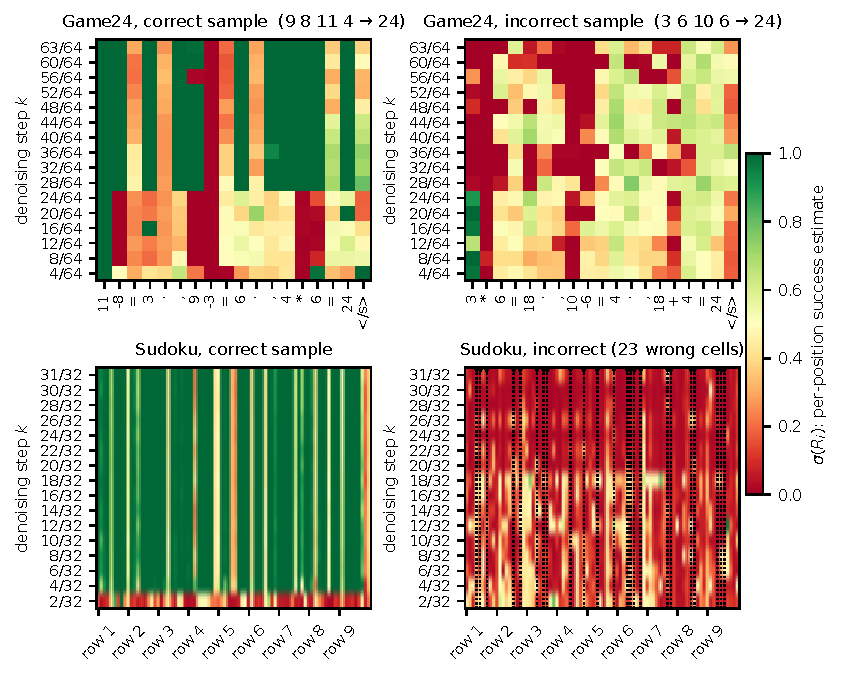
\includegraphics[width=0.58\linewidth]{figures/fig_critic_maps.pdf}
\caption{Per-position critic readings $r_{k,i}$ (colour) along the deployment-sampler trajectory (rows: denoising step $k$; columns: generated positions, labelled by the decoded token for Game24 and by Sudoku row) for one correct and one incorrect held-out sample per task. The correct samples are the median-valued correct rollout; the incorrect Game24 sample is the median-valued failed rollout and the incorrect Sudoku sample the failed rollout with the fewest wrong cells (dotted lines and markers).}
\label{fig:critic_maps}
\end{figure}

\subsubsection{1D against 2D critic over training, all tasks}
\label{app:traj}
Figure~\ref{fig:traj} extends the left panel of Figure~\ref{fig:dyn} from Game24 to the four tasks and adds the AUC of the jointly trained head. On Game24 and K\&K both heads keep up with the policy and the 2D critic's policy climbs further; on Countdown the pooled head falls behind the moving policy and its policy turns back; on Sudoku both heads keep their AUC while both policies turn back early, the 2D critic's later and from a higher peak.

\begin{figure}[!t]
\centering
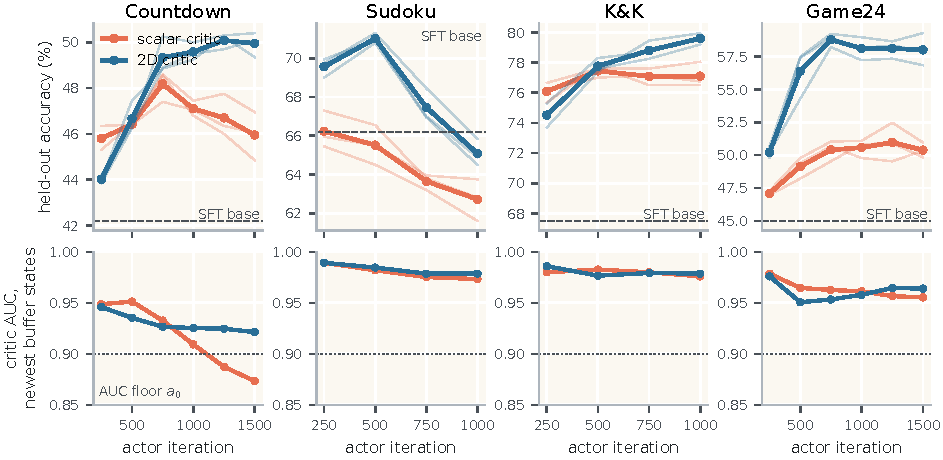
\includegraphics[width=0.85\linewidth]{figures/fig_traj.pdf}
\caption{1D against 2D critic over training: the runs of Table~\ref{tab:main}, individual runs (thin) and their mean (thick). Top: held-out accuracy (\%) at the deployment sampler of the checkpoint after that many actor iterations; dashed: the SFT base. Bottom: AUC of the jointly trained head against the outcome on the newest 256 replay-buffer states, averaged over 250-iteration windows of the training logs; dotted: the floor $a_0=0.9$ below which Algorithm~\ref{alg:jpc} gives the critic extra steps. Bottom-row curves are means over the runs. On Countdown the pooled head falls behind the moving policy and its policy turns back; on Sudoku both heads keep their AUC and the 1D critic's policy declines from the start; on Game24 and K\&K both heads keep up and the 1D critic's gain is smaller.}
\label{fig:traj}
\end{figure}

\subsubsection{The 1D and the 2D critic are interchangeable at a fixed policy}
\label{app:critic_equiv}
Table~\ref{tab:critic_equiv} compares the pre-trained 1D and 2D critics of the Table~\ref{tab:main} runs on the same states of the same policy, and their jointly trained heads on fixed probe sets. Measured this way the two critics discriminate the reward equally well, prescribe parameter updates at cosine $0.83$--$0.90$ of each other, react equally, and weakly, to a single wrong token, and their heads refit equally stably. None of the fixed-policy measurements separates the two critics: whatever distinguishes the policies they train (Figures~\ref{fig:dyn} and~\ref{fig:traj}) is not visible in either critic's value, slope or stability at a fixed policy, which is why we attribute the difference to the joint training rather than to what the critics can represent.

\begin{table}[!t]\centering\small
\caption{1D against 2D critic on the same states. Pre-trained critics unless a row says otherwise; $k$ is the denoising step of the state.}\label{tab:critic_equiv}
\footnotesize\setlength{\tabcolsep}{3pt}
\begin{tabular}{@{}p{0.35\linewidth}p{0.20\linewidth}>{\raggedright\arraybackslash}p{0.20\linewidth}>{\raggedright\arraybackslash}p{0.20\linewidth}@{}}\toprule
measurement & setting & 1D & 2D\\\midrule
Pearson correlation of the pooled value with the outcome, held-out rollouts & pre-training, Game24 $k{=}48$ / Sudoku $k{=}18$ / Countdown $k{=}14$ & 0.97 / 0.94 / 0.99 & 0.97 / 0.94 / 0.99\\
pathwise SNR of the actor's parameter gradient (Table~\ref{tab:snr} statistic) & Game24 $k{=}16$ / 24 / 32 & 0.19 / 0.17 / 0.20 & 0.18 / 0.18 / 0.15\\
half-split cosine of the actor's parameter gradient & Game24 $k{=}16$ / 24 / 32 & 0.81 / 0.78 / 0.83 & 0.81 / 0.79 / 0.70\\
cosine between the two critics' mean actor gradients & Game24 $k{=}16$ / 24 / 32 & \multicolumn{2}{l}{0.90 / 0.88 / 0.83}\\
cosine between the two critics' per-position gradient-norm profiles & Game24, real tokens & \multicolumn{2}{l}{0.94 / 0.94 / 0.94}\\
mean pairwise cosine of per-position state gradients $\partial V_\phi/\partial\rvz_{t_k}[i]$ (shared direction) & Game24 $k{=}24$ / Sudoku $k{=}12$ & 0.03 / 0.06 & 0.04 / 0.07\\
pooled $\Delta V_\phi$ (logits) for one wrong token in a successful state & Game24 $k{=}24$, re-encoded & $-0.86$ & $-0.89$\\
\quad the same, corruptions that break the answer & Game24 $k{=}24$ & $-1.76$ & $-2.04$\\
pooled $\Delta V_\phi$ for one wrong cell (never changes the decoded grid) & Sudoku $k{=}12$ & $-0.11$ & $-0.03$\\
jointly trained head: AUC on states of its own peak policy, iteration 0 $\to$ end & Game24 / Sudoku / Countdown & 0.97$\to$0.96 / 0.98$\to$0.98 / 0.90$\to$0.92 & 0.96$\to$0.96 / 0.98$\to$0.98 / 0.90$\to$0.91\\
jointly trained head: AUC on the newest buffer states, mean over training & Game24 / Sudoku / K\&K / Countdown & 0.96 / 0.98 / 0.98 / 0.92 & 0.96 / 0.98 / 0.98 / 0.93\\
actor gradient after 20 head refits: cosine to the gradient before them & Game24 $k{=}32$, buffer displaced 5\%/refit & 0.98 & 0.99\\
\bottomrule\end{tabular}\end{table}

% ---- CUT 2026-09-26 (not needed for the main narrative): State-gradient profiles of the 1D and the 2D critic ----
\iffalse
\subsubsection{State-gradient profiles of the scalar and the 2D critic}
\label{app:actor_signal}
Table~\ref{tab:actor_signal} reads the actor's instruction $g_i=\partial V_\phi/\partial y_{k,i}$ for the pre-trained scalar and 2D Game24 critics on the same 256 states of the SFT policy under the deployment chain, restricted to the real tokens of each response (18 of 64 generated positions on average). Top-10\% share: fraction of $\sum_i\|g_i\|^2$ on the 10\% of positions with the largest norm (uniform baseline $0.11$). Spearman: rank correlation across positions between $\|g_i\|$ and the undecidedness of position $i$, the negative margin between the decoder's top two logits at $\hat x_{k-1,i}$. The two critics' profiles agree at cosine $0.94$ (Spearman $0.90$) at every step: the order of head and mean does not change where the signal lands on the state, so the 2D critic's gain in Table~\ref{tab:main} is not a redistribution of the actor's signal over positions. For both critics about three quarters of the squared norm of $\nabla_{\theta}V_\phi$ flows through the estimate channel $\hat x_{k-1}$ of~(\ref{eq:chainrule}) rather than through the re-noised state, which supports reading the estimate (Section~\ref{sec:critic}).
\begin{table}[H]\centering\small
\caption{Per-position actor signal on Game24 (real tokens; mean over 256 states).}\label{tab:actor_signal}
\begin{tabular}{@{}llccc@{}}\toprule
 & & $k=16$ & $k=24$ & $k=32$\\\midrule
\multirow{2}{*}{top-10\% share of $\sum_i\|g_i\|^2$} & scalar critic & 0.43 & 0.45 & 0.45\\
 & 2D critic & 0.44 & 0.45 & 0.45\\\midrule
\multirow{2}{*}{Spearman$(\|g_i\|,\ \text{undecidedness})$} & scalar critic & 0.61 & 0.60 & 0.59\\
 & 2D critic & 0.64 & 0.64 & 0.60\\\midrule
\multirow{2}{*}{share of the signal through the estimate channel $\hat x_{k-1}$} & scalar critic & 0.79 & 0.79 & 0.79\\
 & 2D critic & 0.77 & 0.77 & 0.77\\\midrule
cosine of the two critics' $\|g_i\|$ profiles & & 0.94 & 0.94 & 0.94\\\bottomrule\end{tabular}\end{table}

\fi


% ---- CUT 2026-09-26 (not needed for the main narrative): Exchanging the critics (late exchanges) ----
\iffalse
\subsubsection{Exchanging the critics}
\label{app:swap_late}
In the right panel of Figure~\ref{fig:dyn} the scalar critic's policy handed to the 2D critic at iteration 250 climbs to within a point of the run that had the 2D critic throughout, and the 2D critic's policy handed to the scalar critic stops where the scalar runs stop; the critic in charge for the rest of the schedule decides where the run ends, not the policy it starts from.
Table~\ref{tab:swap} gives the values behind the right panel of Figure~\ref{fig:dyn}: a run of each recipe is stopped at iteration 250 and continued for the rest of the same schedule (cosine $0.94\times10^{-6}\to10^{-7}$ over the remaining 1{,}250 iterations) with its own critic or with the other recipe's pre-trained critic, whose head is refit from iteration 250 on as in Algorithm~\ref{alg:jpc}. \begin{table}[H]\centering\small
\caption{Exchanging the critics on Game24. Each cell is the held-out accuracy (\%) at the deployment sampler after that many actor iterations in total.}\label{tab:swap}
\begin{tabular}{@{}llcccccc@{}}\toprule
policy at iteration 250 & critic from 250 on & 250 & 500 & 750 & 1000 & 1250 & 1500 \\\midrule
trained with the scalar critic & scalar (unchanged) & 47.7 & 49.8 & 51.6 & 49.8 & 49.9 & 50.8 \\
 & 2D (exchanged) & 47.7 & 51.3 & 51.5 & 54.2 & 55.8 & 56.4 \\\midrule
trained with the 2D critic & 2D (unchanged) & 49.8 & 52.3 & 52.4 & 56.1 & 56.7 & 57.3 \\
 & scalar (exchanged) & 49.8 & 51.7 & 51.8 & 50.1 & 50.1 & 51.3 \\
\bottomrule\end{tabular}\end{table}
The exchange above is made while the policy is still moving. Table~\ref{tab:swap_late} makes it at iteration 750 instead, from the 2D-critic run of Table~\ref{tab:main} at iteration 750, continuing for 750 more iterations at a learning rate that has already decayed (cosine $5\times10^{-7}\to10^{-7}$) with either the 2D or the scalar critic, pre-trained and refit as in Algorithm~\ref{alg:jpc}. The two continuations are indistinguishable and both stay within two points of their starting point: once the policy has reached its plateau and the step size is small, the pooled value is no longer a shortcut the actor can take, and the field has nothing left to add. The difference between the two critics is made while the policy moves.
\begin{table}[H]\centering\small
\caption{Late exchange on Game24. The 2D-critic policy at iteration 750 (held-out $58.2$) is continued for 750 more iterations with either critic; held-out accuracy (\%) at the deployment sampler after that many further iterations.}\label{tab:swap_late}
\begin{tabular}{@{}lccc@{}}\toprule
critic from iteration 750 on & +250 & +500 & +750\\\midrule
2D & 57.5 & 56.7 & 57.3\\
scalar & 57.0 & 56.4 & 56.2\\
\bottomrule\end{tabular}\end{table}

\fi


\subsubsection{Frozen versus joint critic}
\label{app:frozen}
The right panel of Table~\ref{tab:critic_design} shows the exploit directly on Game24: the recipe of Algorithm~\ref{alg:jpc} with the pre-trained 2D critic held fixed. The pathwise update first helps, then the actor finds the critic's blind spots: the critic's value on the training batch climbs from about $3$ logits at iteration 250 to over $80$ by 1500 while the true success rate of the same batch falls from $78\%$ to $0\%$, and the held-out accuracy collapses. The identical run with the head refit after every actor step (Table~\ref{tab:main}) keeps the critic's value in the calibrated range. Increasing the frozen critic's quality (more pre-training rollouts, the 2D form) does not change this: whatever the critic is, the actor exploits it within a few hundred updates unless the critic is refreshed on the actor's own states.

% ---- CUT 2026-09-26 (not needed for the main narrative): Which parts of the critic are trained, and from where ----
\iffalse
\subsubsection{Which parts of the critic are trained, and from where}
\label{app:critic_training}
Table~\ref{tab:critic_training} separates the two choices behind the critic of Algorithm~\ref{alg:jpc}: that its network starts as a copy of the denoiser, and that during RL only its head is refit. All four runs share the frozen text encoder, the actor, the critic architecture, the pre-training rollouts and epochs, and the head refit of Algorithm~\ref{alg:jpc}; they differ only in how the critic's network is initialised before pre-training and in whether it receives gradients during RL (learning rate $10^{-5}$, that of pre-training). Training the copy during RL costs eight points and its gain does not carry to the cheap chain ($33.6$ against $35.4$ for the base). A randomly initialised network, pre-trained on the same rollouts, reads the outcome only weakly (Table~\ref{tab:critic_design}) and takes the policy below the base. Training it during RL then acts as a stabiliser and not as a remedy: with its network frozen the weak critic is exploited to collapse, the same collapse as the frozen critic in the right panel of Table~\ref{tab:critic_design}, and with its network trained the policy settles twelve points under the base.
\begin{table}[H]\centering\small
\caption{How the critic's network is obtained and trained (Game24, Algorithm~\ref{alg:jpc} otherwise). Each cell is the held-out accuracy (\%) at the deployment sampler after that many actor iterations; the base is $45.0$. The random initialisation resets every attention, feed-forward and embedding weight of the network; its few learned prefix tokens and normalisation gains keep their values. Blue: the critic of Algorithm~\ref{alg:jpc}.}\label{tab:critic_training}
\begin{tabular}{@{}llcccccc@{}}\toprule
network before pre-training & network during RL & 250 & 500 & 750 & 1000 & 1250 & 1500 \\\midrule
\hl{copy of the denoiser} & \hl{frozen} & 49.8 & 57.2 & 58.2 & 56.2 & 56.5 & 57.5 \\
copy of the denoiser & trained & 47.2 & 49.7 & 47.3 & 47.4 & 48.8 & 49.3 \\
random & trained & 39.2 & 35.4 & 34.2 & 33.5 & 33.4 & 33.4 \\
random & frozen & 37.9 & 24.2 & \phantom{0}1.4 & \phantom{0}0.8 & \phantom{0}2.6 & \phantom{0}4.1 \\
\bottomrule\end{tabular}\end{table}

\fi


% ---- CUT 2026-09-26 (not needed for the main narrative): Ablations: full checkpoint trajectories ----
\iffalse
\subsubsection{Ablations: full checkpoint trajectories}
\label{app:needs_full}
Table~\ref{tab:needs_full} gives every evaluated checkpoint behind Table~\ref{tab:needs}. The probability objective and minimum pooling stay below the reference at every checkpoint, and training under the cheap chain stays below it at deployment throughout. The five-step buffer of block B was also run on Countdown, where the outcome is not readable before the middle of the chain (held-out AUC $0.64$ at steps 8--24 against $0.90$ at step 40): there it costs over two points against the single-step buffer of Algorithm~\ref{alg:jpc} with the same pre-trained critic ($47.9$ against $50.2$ at the deployment sampler), which is why the recipe refits at $k_{\rm hi}$.

The per-position loss term is the one choice whose ablation depends on the task. On Game24, refitting the 2D critic with the pooled term of~(\ref{eq:critic2d_loss}) alone changes nothing. On Countdown, where the scalar critic's head falls behind its policy (Appendix~\ref{app:traj}), the same ablation removes the 2D critic's advantage (block A): the runs peak at about $47$ and end at about $45$, against end values of about $50$ with both terms and $45.4$ for the scalar critic. Its head also degrades as the scalar head does: the in-sample AUC of the last 250 iterations is $0.88$ against $0.91$--$0.93$ with both terms, and the AUC check fires in $20$--$21$ of the last $25$ tests against $0$--$8$. More refit does not help the scalar critic either. With $m_{\rm c}{=}8$ head steps per actor step in place of $2$, the scalar-critic runs end at $42$--$46$, no better than with two steps, and the head's in-sample AUC falls faster ($0.83$ in the last 250 iterations, the check firing every time). The scalar critic's stall on Countdown is thus not a matter of refit budget, and the order of head and mean alone does not remove it; what does is fitting every reading to the outcome, the constraint Section~\ref{sec:jpc_2d} introduces the second term for.
\begin{table}[H]
\centering\small
\caption{Full checkpoint trajectories of the ablations of Table~\ref{tab:needs}. Each cell is the held-out accuracy (\%) at the deployment sampler of the checkpoint saved after that many actor iterations; \emph{best} is the highest cell of the row (for rows that average several runs, the mean of their per-run maxima); the SFT base is $45.0$. Rows are single runs unless the number of runs is given, and then the cells are means over them. Blocks A--C are the recipe versions of Appendix~\ref{app:details}; block A stands behind rows 1--2 of Table~\ref{tab:needs} and block C behind row 3; reference rows are means over three runs. Blue: recommended variant; bold: the highest cell of the row.}
\label{tab:needs_full}
\scriptsize\setlength{\tabcolsep}{3pt}
\begin{tabular}{@{}>{\raggedright\arraybackslash}p{0.17\linewidth}>{\raggedright\arraybackslash}p{0.34\linewidth}cccccc|c@{}}
\toprule
choice it tests & variant & \multicolumn{6}{c}{accuracy after $n$ actor iterations} & best \\
 & & $n{=}250$ & 500 & 750 & 1000 & 1250 & 1500 & \\
\midrule
\multicolumn{9}{@{}l}{\emph{A. Algorithm~\ref{alg:jpc} (single-step buffer, both loss terms, AUC check, cosine decay)}}\\
 & \hl{reference (3 seeds)} & 50.2 & 56.4 & 58.8 & 58.1 & 58.1 & 58.0 & \textbf{58.8} \\
Section~\ref{sec:pathwise}, objective & actor ascends $\mathrm{sig}(V_\phi)$ instead of $V_\phi$ & \ABp{1} & \ABp{2} & \ABp{3} & \ABp{4} & \ABp{5} & \ABp{6} & \ABp{7} \\
Section~\ref{sec:jpc_2d}, pooling & actor ascends $\min_iR_{k,i}$ instead of the mean & \ABm{1} & \ABm{2} & \ABm{3} & \ABm{4} & \ABm{5} & \ABm{6} & \ABm{7} \\
 & \emph{Countdown:} reference (3 seeds; base $42.2$) & 44.0 & 46.6 & 49.3 & 49.6 & 50.1 & 50.0 & 50.2 \\
Section~\ref{sec:pathwise}, objective & \emph{Countdown:} actor ascends $\mathrm{sig}(V_\phi)$ & \ABcp{1} & \ABcp{2} & \ABcp{3} & \ABcp{4} & \ABcp{5} & \ABcp{6} & \ABcp{7} \\
 & \emph{Countdown:} reference (2 runs) & 44.2 & 47.3 & 49.8 & 49.9 & 49.4 & 50.2 & 50.4 \\
Section~\ref{sec:jpc_2d}, supervision & \emph{Countdown:} pooled loss term only (2 runs) & 44.2 & 44.0 & 45.8 & 46.4 & 45.8 & 44.8 & 46.9 \\
 & \emph{Countdown:} scalar critic, $m_{\rm c}{=}2$ (3 runs) & 45.8 & 46.4 & 48.2 & 47.1 & 46.7 & 45.9 & 48.2 \\
Section~\ref{sec:joint}, critic ahead of actor & \emph{Countdown:} scalar critic, $m_{\rm c}{=}8$ (2 runs) & 42.8 & 44.5 & 43.8 & 44.5 & 44.1 & 43.8 & 44.9 \\
\midrule
\midrule
\multicolumn{9}{@{}l}{\emph{C. 1000 iterations, constant learning rate $10^{-6}$, five-step buffer}}\\
 & reference & 48.7 & 50.9 & 53.0 & 56.4 & --- & --- & 56.4 \\
Section~\ref{sec:joint}, critic must move & critic frozen after pre-training & 48.4 & 48.0 & \phantom{0}2.1 & \phantom{0}0.3 & --- & --- & 48.4 \\
Section~\ref{sec:joint}, critic ahead of actor & $m_{\rm c}{=}1$ head step per actor step & 48.0 & 51.7 & 48.6 & 51.1 & --- & --- & 51.7 \\
 & $m_{\rm c}{=}8$ & 47.0 & 52.3 & 54.7 & 55.2 & --- & --- & 55.2 \\
Section~\ref{sec:joint}, staleness & buffer $N_{\mathcal B}{=}4$k instead of 16k & 47.8 & 50.1 & 52.6 & 56.4 & --- & --- & 56.4 \\
Section~\ref{sec:joint}, one chain & trained under $\gamma4$@16, read at $\gamma56$@64 & 44.7 & 44.3 & 41.5 & 47.0 & --- & --- & 47.0 \\
 & \quad the same run read at $\gamma4$@16 (base $35.4$) & 35.1 & 38.7 & 41.3 & 42.5 & --- & --- & 42.5 \\
\bottomrule
\end{tabular}
\end{table}

\fi


\subsubsection{Training dynamics on Countdown and K\&K}
\label{app:dynamics}
Figure~\ref{fig:dynamics_cd_kk} shows the Algorithm~\ref{alg:jpc} runs with the 2D critic on the two tasks not covered by Figure~\ref{fig:dyn}. On Countdown the held-out accuracy rises for about 750 iterations and then holds while the replay-buffer success rate keeps climbing: the training batch keeps improving after the held-out set has levelled off. On K\&K the held-out accuracy rises monotonically and is still at its peak when the schedule ends; its buffer success rate and critic value rise together over the whole run.

% ---- CUT 2026-09-26 (not needed for the main narrative): Figure with the Game24 loop check ----
\iffalse
\begin{figure}[H]
\centering
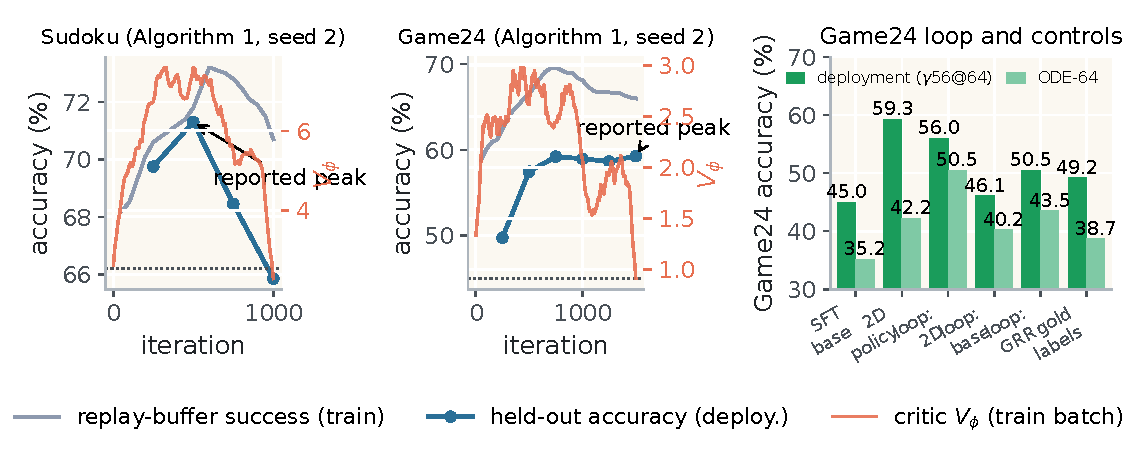
\includegraphics[width=\linewidth]{figures/fig_dynamics_loop.pdf}
\caption{Left, middle: two Algorithm~\ref{alg:jpc} runs (2D critic, cosine $10^{-6}\!\to\!10^{-7}$): replay-buffer success (grey), critic value on the training batch (red) and held-out accuracy at the deployment sampler (blue).Right: the Game24 rounds and their controls at the deployment and ODE-64 samplers (base; 2D-critic policy; four plain rounds from that policy, from the base, from the GRPO policy, and on gold labels), the check of Appendix~\ref{app:g24_loop}.}
\label{fig:curves}
\end{figure}
\fi

\begin{figure}[H]
\centering
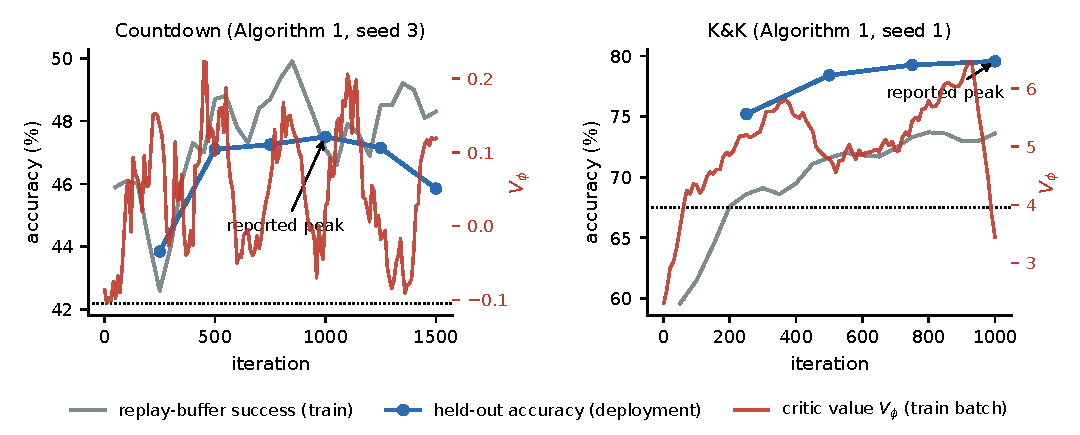
\includegraphics[width=0.85\linewidth]{figures/fig_dynamics_cd_kk.pdf}
\caption{Training dynamics of Algorithm~\ref{alg:jpc} (2D critic) on Countdown (left) and K\&K (right): held-out accuracy at the deployment sampler per checkpoint (blue), replay-buffer success rate (grey), and the critic's value on the training batch (red, right axis); dotted line: SFT base.}
\label{fig:dynamics_cd_kk}
\end{figure}

\subsection{The loop}
This group stands behind Table~\ref{tab:loop}: every round of every loop with its controls, and the critic-guided sampler that draws the later Countdown rounds.

\subsubsection{The loop in full: rounds, controls and the guided sampler}
\label{app:loop_full}
Table~\ref{tab:loop_full} gives every round behind Table~\ref{tab:loop} with the pool's coverage and the controls. On Countdown and K\&K the rounds lift the cheap sampler by 17 to 35 points from every start, RL or not. On K\&K fresh puzzles give near-full coverage from any start and the rounds close the task; RL adds nothing there that the rounds do not. On Sudoku one round covers three quarters of the pool from every start and moves accuracy by at most 1.4 points at either sampler, as the gold-solution control confirms. On Countdown two plain rounds shrink coverage and give back part of the RL gain; rounds 3 and 4, drawn with the critic-guided cheap sampler, raise coverage past its start and return the deployment sampler to the RL level, 5 to 7 points above sampling plainly from the base or the \methodGRPO{} policy. Two further plain rounds continued from the round-2 model (the two control rows after round 4) leave coverage and accuracy at the round-2 level, whereas the critic-guided rounds from the same model cover about six thousand more problems and recover $4.5$--$5.9$ points at deployment; the recovery is therefore due to the critic-guided pools, not to the additional rounds. 

% Table~\ref{tab:guided} isolates the guided sampler on the first $5{,}000$ pool problems with the loop's starting policy and its jointly trained critic at $\gamma4$@16: pruning four trajectories at random changes nothing; pruning them by the critic's minimum reading~(\ref{eq:minscore}) doubles the acceptance rate and raises coverage by a third, and the push~(\ref{eq:guide}) adds to both.

\begin{table}[H]
\centering\small
\caption{The amortization loop, held-out accuracy (\%) at three samplers. Each block is one task: the SFT base, the 2D-critic policy the loop starts from, the model at the end of each round of Algorithm~\ref{alg:loop} (Countdown: all four rounds; K\&K: first and last of five; Sudoku: its one round), and, indented, the controls at their last round, which run the same rounds without a critic from the SFT base, from the \methodGRPO{} policy, and on the gold derivations of the same pool, and, for Countdown, two further plain rounds continued from the round-2 model. \emph{Covered}: pool problems (of 50k) with at least one verified sample in that round. Game24 has no pool of unlabelled problems. Sudoku's cheap sampler is $\gamma14$@16 and its deployment sampler $\gamma28$@32. Bold: the last round of each loop where it is over 1.0 point above the start.}
\label{tab:loop_full}
\setlength{\tabcolsep}{4.5pt}
\begin{tabular}{@{}llcccc@{}}
\toprule
 & pool sampler & covered & 16-step sampler & ODE-64 & deployment \\
\midrule
\multicolumn{6}{@{}l}{\emph{Countdown}}\\
SFT base & & & 23.8 & 28.5 & 42.8 \\
2D-critic policy (start) & & & 24.3 & 34.8 & 50.5 \\
round 1 & deployment sampler & 35.1k & 37.9 & 42.4 & 45.8 \\
round 2 & deployment sampler & 31.2k & 40.8 & 42.6 & 46.0 \\
round 3 & critic-guided, $\gamma4$@16 & 37.2k & \OURScdthreeg & \OURScdthreeo & \OURScdthree \\
round 4 & critic-guided, $\gamma4$@16 & 37.8k & \textbf{\OURScdg} & \textbf{\OURScdo} & \OURScd \\
\quad plain round 3 (control) & deployment sampler & 31.2k & 41.1 & 43.7 & 45.5 \\
\quad plain round 4 (control) & deployment sampler & 31.3k & 41.1 & 43.4 & 45.5 \\
\quad control: from the SFT base & deployment sampler & 31.2k & 42.7 & 44.5 & 46.4 \\
\quad control: from \methodGRPO{} & deployment sampler & 30.9k & 41.1 & 42.9 & 44.7 \\
\quad control: gold derivations & (labels) & 50.0k & 22.5 & 26.4 & 40.8 \\
\midrule
\multicolumn{6}{@{}l}{\emph{K\&K}}\\
SFT base & & & 58.6 & 57.5 & 68.2 \\
2D-critic policy (start) & & & 68.8 & 69.7 & 79.8 \\
round 1 & deployment sampler & 41.1k & 73.4 & 76.6 & 82.1 \\
round 5 & deployment sampler & 48.8k & \textbf{\OURSkkg} & \textbf{\OURSkko} & \textbf{\OURSkk} \\
\quad control: from the SFT base & deployment sampler & 49.4k & 93.5 & 97.0 & 99.6 \\
\quad control: from \methodGRPO{} & deployment sampler & 48.3k & 91.7 & 94.6 & 97.9 \\
\quad control: gold labels & (labels) & 50.0k & 94.8 & 98.0 & 99.6 \\
\midrule
\multicolumn{6}{@{}l}{\emph{Sudoku}}\\
SFT base & & & 60.0 & 60.6 & 64.0 \\
2D-critic policy (start) & & & 63.4 & 65.3 & 68.9 \\
round 1 & deployment sampler & 39.3k & 63.1 & 65.4 & \textbf{70.3} \\
\quad control: from the SFT base & deployment sampler & 36.1k & 58.7 & 60.7 & 63.6 \\
\quad control: from \methodGRPO{} & deployment sampler & 39.3k & 64.2 & 67.7 & 69.6 \\
\quad control: gold solutions & (labels) & 50.0k & 63.9 & 65.2 & 69.7 \\
\bottomrule
\end{tabular}
\end{table}

% \begin{table}[H]
% \centering\small
% \caption{The critic as a search heuristic. Each row is one way of drawing samples from the Countdown 2D-critic policy the loop starts from (Table~\ref{tab:loop_full}) and its jointly trained critic at $\gamma4$@16 on the first 5{,}000 pool problems, four samples per problem: \emph{acc.}, the fraction of samples the verifier accepts; \emph{coverage}, problems (of 5{,}000) with at least one accepted sample; \emph{distinct}, distinct accepted derivations.}
% \label{tab:guided}
% \begin{tabular}{@{}lccc@{}}
% \toprule
% sampler & acc.\ (\%) & coverage & distinct \\
% \midrule
% plain & \GBa{1} & \GBa{2} & \GBa{3} \\
% best of 4 at step 8, random & \GBb{1} & \GBb{2} & \GBb{3} \\
% best of 4 at step 8, by the critic & \GBc{1} & \GBc{2} & \GBc{3} \\
% push~(\ref{eq:guide}) at every step & \GBd{1} & \GBd{2} & \GBd{3} \\
% best of 4 by the critic + push & \GBe{1} & \GBe{2} & \GBe{3} \\
% \bottomrule
% \end{tabular}
% \end{table}

% ---- CUT 2026-09-26 (not needed for the main narrative): Cheap samplers after the loop ----
\iffalse
\subsubsection{Cheap samplers after the loop}
\label{app:samplers}
Table~\ref{tab:samplers} reads one 2D-critic checkpoint per task and its loop across sampler cost. RL alone moves Countdown's cheap samplers little ($+0.5$ at $\gamma4$@16 against $+7.7$ at deployment), whereas on K\&K and Sudoku the RL gain carries to every sampler. One loop moves the rest: after it, the 16-step sampler reaches or passes the accuracy the 64-step deployment sampler had before RL on Countdown and K\&K ($\OURScdg$ vs $42.8$, $\OURSkkg$ vs $68.2$), and on K\&K it passes the deployment accuracy of the RL policy itself ($\OURSkkg$ vs $79.8$). Sudoku, whose loop is null, moves by at most 1.4 points at any sampler; Game24 has no loop (Appendix~\ref{app:g24_loop}).

\begin{table}[H]\centering\small
\caption{The loop moves what the policy can do to the cheap samplers. Held-out accuracy (\%) at samplers of increasing cost: the SFT base, the 2D-critic policy and the model after the loop (final round). $^\dagger$On Sudoku this column is $\gamma14$@16 and the deployment column is $\gamma28$@32. Bold: the best row of each block; blue: recommended variant.}\label{tab:samplers}
\begin{tabular}{@{}llcccc@{}}\toprule
 & & $\gamma4$@16 & $\gamma28$@32$^\dagger$ & ODE-64 & deployment\\\midrule
\multirow{3}{*}{Countdown} & SFT base & 23.8 & 38.1 & 28.5 & 42.8\\
 & 2D-critic policy & 24.3 & 43.9 & 34.8 & 50.5\\
 & \hl{+ loop} & \textbf{45.6} & \textbf{51.1} & \textbf{47.8} & \textbf{51.4}\\\midrule
\multirow{3}{*}{Sudoku} & SFT base & 52.5 & 60.0 & 60.6 & 64.0\\
 & 2D-critic policy & \textbf{54.2} & \textbf{63.4} & 65.3 & 68.9\\
 & \hl{+ loop} & 53.7 & 63.1 & \textbf{65.4} & \textbf{70.3}\\\midrule
\multirow{3}{*}{K\&K} & SFT base & 58.6 & 66.3 & 57.5 & 68.2\\
 & 2D-critic policy & 68.8 & 76.3 & 69.7 & 79.8\\
 & \hl{+ loop} & \textbf{93.8} & \textbf{97.9} & \textbf{95.7} & \textbf{99.1}\\\midrule
\multirow{2}{*}{Game24} & SFT base & 35.6 & 43.5 & 36.2 & 44.0\\
 & 2D-critic policy & \textbf{38.9} & \textbf{54.2} & \textbf{43.5} & \textbf{59.6}\\
\bottomrule\end{tabular}\end{table}

\fi


% ---- CUT 2026-09-26 (not needed for the main narrative): Countdown loop round by round ----
\iffalse
\subsubsection{Countdown loop round by round}
\label{app:cd_loop}
Table~\ref{tab:cd_loop} lists every round of the Countdown loop at all four samplers, together with three of the controls of Table~\ref{tab:loop_full}, which run the same four rounds from the SFT base, from the GRPO policy, and from the 2D policy on the gold labels of the same pools. Three regularities are visible. (i) The loop transfers the policy's ability to the cheap samplers at once: one round takes the ODE sampler from $34.8$ to $42.4$ and $\gamma4$@16 from $24.3$ to $37.9$ while the deployment sampler gives back nearly 5 points. (ii) Plain self-sampling loses ground at the deployment sampler ($50.5\to45.8\to46.0$) and the pool's coverage shrinks (35.1k to 31.2k solved problems). (iii) Sampling the pool with the jointly trained 2D critic (best-of-4 pruning at the midpoint of the 16-step chain plus gradient guidance, Appendix~\ref{app:details}) restores coverage and lifts the deployment sampler ($\OURScdthree$ after round 3, $\OURScd$ after round 4). The plain chains from the base and from the GRPO policy show the first two regularities and stop at $45$--$46$; the gold-label chain falls from $50.5$ to $45.5$ in its first round and drifts to $40.8$ by round 4 (ODE-64 from $34.8$ to $26.4$): fine-tuning the RL policy on gold derivations undoes part of what RL changed rather than adding to it.

\begin{table}[H]\centering\small
\caption{Countdown amortisation loop, held-out accuracy at the end of each round (20 epochs of fine-tuning per round; verifier-accepted sequences and distinct problems in each pool). From top: loop from the 2D-critic policy (Table~\ref{tab:loop}); from the SFT base with no RL; from the GRPO policy; from the 2D-critic policy on the gold labels of the same pools.}\label{tab:cd_loop}
\scriptsize\setlength{\tabcolsep}{2.5pt}
\begin{tabular}{@{}llcccc@{}}\toprule
round & pool & ODE-64 & $\gamma4$@16 & $\gamma28$@32 & $\gamma56$@64\\\midrule
SFT base (epoch 60) & & 28.5 & 23.8 & 38.1 & 42.8\\
\methodSVGTwoD{} policy (start) & & 34.8 & 24.3 & 43.9 & 50.5\\
round 1 & deployment sampler, 91.9k sequences / 35.1k problems & 42.4 & 37.9 & 45.0 & 45.8\\
round 2 & deployment sampler, 57.4k / 31.2k & 42.6 & 40.8 & 45.3 & 46.0\\
round 3 & 2D-critic-guided sampler, \OURSpoolthree & \OURScdthreeo & \OURScdthreeg & \OURScdthreet & \OURScdthree\\
round 4 & 2D-critic-guided sampler, \OURSpoolfour & \OURScdo & \OURScdg & \OURScdt & \OURScd\\\midrule
no-RL round 1 & deployment sampler, 82.4k / 34.2k & 40.1 & 34.4 & 44.8 & 46.6\\
no-RL round 2 & 59.1k / 30.8k & 42.0 & 39.9 & 45.5 & 46.8\\
no-RL round 3 & 52.2k / 30.8k & 43.7 & 43.3 & 45.8 & 46.1\\
no-RL round 4 & 48.5k / 31.2k & 44.5 & 42.7 & 46.3 & 46.4\\\midrule
GRPO policy (start) & & 29.5 & 23.7 & 40.1 & 43.0\\
GRPO round 1 & deployment sampler, 82.7k / 34.1k & 42.7 & 39.0 & 44.8 & 46.0\\
GRPO round 2 & 58.3k / 30.5k & 43.0 & 39.8 & 45.7 & 47.1\\
GRPO round 3 & 51.3k / 30.4k & 45.2 & 41.2 & 45.7 & 47.1\\
GRPO round 4 & 47.2k / 30.9k & 42.9 & 41.1 & 44.2 & 44.7\\\midrule
gold round 1 & gold derivations, 50k / 50k & 28.2 & 24.6 & 40.2 & 45.5\\
gold round 2 & & 27.1 & 23.5 & 40.1 & 42.0\\
gold round 3 & & 25.8 & 23.2 & 40.4 & 41.0\\
gold round 4 & & 26.4 & 22.5 & 37.6 & 40.8\\\bottomrule\end{tabular}\end{table}

\fi


% ---- CUT 2026-09-26 (not needed for the main narrative): Game24: why there is no loop row ----
\iffalse
\subsubsection{Game24: why there is no loop row}
\label{app:g24_loop}
Game24 is split by number set (Appendix~\ref{app:datasets}): every solvable set is either a training set or a held-out set, so there is no pool of unlabelled problems the policy has not trained on, which is what a round of Algorithm~\ref{alg:loop} needs. Table~\ref{tab:g24_loop} shows what happens when the rounds are run regardless, on the 4{,}693 other orderings of the 1{,}076 training sets, from the 2D-critic policy and from the three control starting points. The starting policy already solves $81\%$ of that pool, so a round mostly re-fits derivations of sets it knows. Read the deployment column against the cheap-sampler columns: the rounds move the ODE and 16-step samplers up by 7 to 11 points, as on the other tasks, while the deployment sampler loses about 3 points in the first round and then holds. Sampling rounds 3--4 with the critic-guided cheap chain of Appendix~\ref{app:loop}, the recipe of the Countdown loop, raises the pool's coverage a little further and lowers every held-out number: the extra accepted derivations are more of the same sets. The gold-label control isolates the cost: fine-tuning the same policy on the gold derivations of the same prompts loses about 10 points at deployment and lowers the cheap samplers by 2 to 5 points, where the self-samples raise them by 7 to 11. What the rounds cost is the supervised fitting of training-set derivations, the effect that already limits the supervised epochs on this task (Appendix~\ref{app:g24_sft}); what they give is the transfer across samplers that the self-samples carry and the gold derivations do not. From the SFT base and from the GRPO policy the rounds gain 2 to 3 points at deployment and 3 to 6 at ODE-64. None of this is the loop of Appendix~\ref{app:loop}, whose gain comes from covering problems the policy does not yet solve, so Table~\ref{tab:loop} carries no Game24 entry.
\begin{table}[H]\centering\small
\caption{Rounds of Algorithm~\ref{alg:loop} on Game24's re-ordered training sets, held-out accuracy (\%) at the end of each round (8 epochs of fine-tuning per round). \emph{Covered}: pool problems with at least one verified sample. From top: from the 2D-critic policy (final checkpoint) with plain deployment-chain sampling, then the same chain continued from round 2 with critic-guided sampling in rounds 3--4; from the SFT base; from the GRPO policy; from the 2D-critic policy on the gold derivations of the same pool.}\label{tab:g24_loop}
\scriptsize\setlength{\tabcolsep}{4pt}
\begin{tabular}{@{}llccc@{}}\toprule
start / round & covered & $\gamma56$@64 & ODE-64 & $\gamma4$@16\\\midrule
\methodSVGTwoD{} policy (start) & & 59.6 & 43.5 & 38.9\\
round 1, plain & 3.79k / 4.69k & 56.8 & 46.9 & 44.2\\
round 2, plain & 3.54k & 56.4 & 49.1 & 48.2\\
round 3, plain & 3.58k & 56.5 & 49.1 & 47.9\\
round 4, plain & 3.64k & 57.0 & 50.5 & 50.2\\
round 3, critic-guided (from round 2) & 3.96k & 55.9 & 48.1 & 48.1\\
round 4, critic-guided & 3.95k & 51.2 & 47.1 & 45.9\\\midrule
SFT base (start) & & 44.0 & 36.2 & 35.6\\
rounds 1--4, plain & & 45.2 / 44.5 / 44.6 / 46.0 & 37.1 / 37.5 / 38.5 / 38.9 & 37.1 / 36.9 / 36.5 / 39.2\\\midrule
GRPO policy (start) & & 48.5 & 37.4 & 36.6\\
rounds 1--4, plain & & 49.4 / 48.5 / 51.7 / 51.2 & 40.0 / 40.9 / 43.1 / 43.2 & 40.5 / 40.6 / 39.6 / 42.1\\\midrule
gold derivations, rounds 1--4 & 4.69k & 54.0 / 50.4 / 49.5 / 48.8 & 38.9 / 38.4 / 39.6 / 39.0 & 39.2 / 36.9 / 36.5 / 36.5\\
\bottomrule\end{tabular}\end{table}

\fi


% ---- CUT 2026-09-26 (not needed for the main narrative): Sampler sweep on the Countdown base model ----
\iffalse
\subsubsection{Sampler sweep on the Countdown base model}
\label{app:sampler_sweep}
Table~\ref{tab:sampler_sweep} records the held-out accuracy of the Countdown SFT model under the samplers we swept before fixing the four reporting samplers. Two regularities hold on every task we tried: at a fixed number of steps $K$ the best $\gamma$ is the one that keeps the per-step retention $\alpha_k$ near $0.125$ (so $\gamma\approx K\cdot0.875$: $\gamma4$@16 is deliberately \emph{below} this and is the cheap sampler; $\gamma14$@16, $\gamma28$@32, $\gamma56$@64 and $\gamma112$@128 are on it), and at that retention more steps keep helping with diminishing returns ($38.1\to42.8\to44.0$ from 32 to 64 to 128 steps). The deployment sampler $\gamma56$@64 is the last point at which the rollout cost is acceptable for RL (64 network evaluations per sample, one of which is recomputed with gradients).

\begin{table}[H]\centering\small
\caption{Countdown held-out accuracy of the SFT model under different samplers (classifier-free guidance 2 unless stated). Left: the base checkpoint used in the paper (epoch 60). Right: an earlier checkpoint (epoch 42) on which the wider grid was run, evaluated on the full held-out set.}\label{tab:sampler_sweep}
\resizebox{\linewidth}{!}{%
\begin{tabular}{@{}lc@{\qquad}lc@{}}\toprule
sampler (epoch 60) & acc. & sampler (epoch 42) & acc.\\\midrule
ODE, 64 steps & 28.5 & ODE, 64 / 128 steps & 23.4 / 24.6\\
$\gamma4$@16 & 23.8 & $\gamma4$@16 / $\gamma14$@16 & 19.9 / 24.1\\
$\gamma28$@32 & 38.1 & $\gamma20$@32 / $\gamma28$@32 / $\gamma28$@32 (guidance 3) & 28.4 / 31.6 / 30.2\\
$\gamma56$@64 (deployment) & 42.8 & $\gamma48$@64 / $\gamma56$@64 / $\gamma56$@64 (guidance 1.5) & 33.8 / 35.0 / 34.9\\
$\gamma112$@128 & 44.0 & $\gamma112$@128 & 37.4\\\bottomrule\end{tabular}}\end{table}


\fi


\section{Related work}
\label{app:related}\label{sec:related}
\paragraph{Continuous-state and diffusion language models.}
Diffusion-LM \citep{li2022diffusionlm} introduced continuous diffusion over word embeddings with per-step rounding; ELF \citep{hu2026elf} shows that removing intermediate discretisation and using flow matching \citep{lipman2022flow,liu2022rectified,albergo2023stochastic} in a frozen T5 embedding space matches autoregressive baselines on translation and summarisation. Masked discrete diffusion \citep{lou2023sedd,sahoo2024mdlm,nie2025llada} is the other line. Its RL methods \citep{zhao2025d1,rojas2026improving,zhu2025llada15} must replace a likelihood the continuous chain has in closed form: the transitions of an observed masked trajectory are tractable, but the marginal likelihood of the decoded sequence sums over trajectories and is not, so they substitute one-step mean-field likelihoods \citep{zhao2025d1} or variational bounds \citep{zhu2025llada15}. Process-aware variants assign step-specific advantages along the denoising trajectory \citep{shao2026papo}, but each advantage is still shared by all token updates of that step.

\paragraph{RL for diffusion and flow models.}
DDPO and DPOK \citep{black2023ddpo,fan2023dpok} cast denoising as an MDP and apply policy gradients to image diffusion; Flow-GRPO, DanceGRPO and MixGRPO \citep{liu2025flowgrpo,xue2025dancegrpo,li2025mixgrpo} extend GRPO to flow matching with ODE-to-SDE conversion, denoising reduction and sliding windows; FPO \citep{mcallister2025fpo} uses the flow-matching loss as a likelihood surrogate inside PPO. Reward back-propagation \citep{prabhudesai2023alignprop,clark2023draft} differentiates a fixed reward model through the sampler, and Adjoint Matching \citep{domingoenrich2024adjoint} frames reward fine-tuning as stochastic optimal control with a memoryless noise schedule. Our update matches ReFL's single-step depth \citep{xu2023imagereward}, but its gradient comes from a jointly trained value of the noisy state rather than a frozen reward on a predicted clean sample, which makes the single step a per-transition estimate rather than a truncation (Appendix~\ref{app:pw_derivation}) and removes the exploitation a frozen reward invites (Table~\ref{tab:critic_design}). Our setting differs in three ways: the reward is a program verifier and not differentiable, so the critic must be learned; the critic is trained jointly; and the pathwise update touches one random step, so nothing is differentiated through the chain.

\paragraph{Actor-critic control.}
Stochastic value gradients \citep{heess2015svg} differentiate a learned value through a reparameterised policy and a transition model; DDPG and SAC \citep{lillicrap2015ddpg,haarnoja2018sac} are the model-free cases. The SVG variants of \method{} are this pattern on a generative chain whose transition model is the sampler itself, with a value that is a success probability fitted to verifier outcomes and, in \methodSVGTwoD{}, a reading per position.

\paragraph{AR post-training.}
RLHF and RLVR \citep{ouyang2022instructgpt,shao2024deepseekmath,deepseek2025r1} use PPO or GRPO \citep{schulman2017ppo,schulman2015gae}; recent variants adjust the clipping and sampling \citep{yu2025dapo,zheng2025gspo}. Their estimator is the score function over categorical decisions, and the reparameterisation alternatives \citep{jang2016gumbel,maddison2016concrete} are biased for categorical actions, which is why the pathwise estimator has no role in AR post-training.

\paragraph{Self-training with verifiers.}
STaR, RFT, ReST-EM and related work \citep{zelikman2022star,yuan2023rft,singh2023restem,huang2022selfimprove} fine-tune a model on its own verified generations; expert iteration \citep{anthony2017exit} alternates a stronger search-based policy with distillation. The amortisation loop is this pattern with an RL policy as the sampler and, in its guided form, with the RL critic as the search heuristic; the controls in Appendix~\ref{app:loop_full} separate what the starting policy contributes from what the rounds contribute. DAV \citep{lee2026dav} casts diffusion alignment as variational expectation-maximisation; a round of Algorithm~\ref{alg:loop} is the M-step of that view for one prompt, with the RL policy as the sampler (Proposition~\ref{prop:em}).

\paragraph{Tasks.}
Countdown and Game24 follow \citet{gandhi2024sos} and \citet{yao2023tot}; Sudoku follows \citet{shah2024sudoku}; Knights-and-Knaves follows \citet{xie2024kk}.

\end{document}
